\documentclass{article}
\usepackage[round]{natbib}
\usepackage{amsmath,amssymb,amsfonts}%
\usepackage{geometry}%
\usepackage{color}
\usepackage{graphicx}
\usepackage{authblk}
\usepackage{nameref}
\usepackage[right]{lineno}
\usepackage{subcaption}
\usepackage{tikz}
\usetikzlibrary{math,calc,positioning}
\usepackage{url}
% JK: turning this off for the moment as I keep clicking through on links
% to the bibliography while reading the text and it's intensely annoying.
% Can reinstate when we're ready to preprint
% \usepackage[hidelinks]{hyperref}

\newcommand{\noderef}[1]{\textsf{#1}}
\newcommand{\tsinfer}[0]{\texttt{tsinfer}}
\newcommand{\kwarg}[0]{\texttt{KwARG}}
\newcommand{\argweaver}[0]{\texttt{ARGweaver}}
\newcommand{\relate}[0]{\texttt{Relate}}
\newcommand{\espalier}[0]{\texttt{Espalier}}

\begin{document}

\linenumbers
\title{A general and efficient representation of Ancestral Recombination Graphs}

% First authors
\author[1]{Yan Wong}

% Second authors
\author[2,$\star$]{Anastasia Ignatieva}
\author[3,4,$\star$]{Jere Koskela}

% Middle Authors
\author[5]{Gregor Gorjanc}
\author[6,7]{Anthony W. Wohns}

% Corresponding
\author[1,$\dagger$]{Jerome Kelleher}

\affil[1]{Big Data Institute, Li Ka Shing Centre for Health Information and Discovery, University of Oxford, OX3 7LF, UK}
\affil[2]{Department of Statistics, University of Oxford, OX1 3LB, UK}
\affil[3]{School of Mathematics, Statistics and Physics, Newcastle University, NE1 7RU, UK}
\affil[4]{Department of Statistics, University of Warwick, CV4 7AL, UK}
\affil[5]{The Roslin Institute and Royal (Dick) School of Veterinary Studies, University of Edinburgh, EH25 9RG, UK}
\affil[6]{Broad Institute of MIT and Harvard, Cambridge, MA 02142, USA}
\affil[7]{Department of Genetics, Stanford University School of Medicine, Stanford, CA 94305, USA}

\affil[$\star$]{Denotes shared second authorship, listed alphabetically}
\affil[$\dagger$]{Denotes corresponding author}


\maketitle

% FIXME this is weak, but gives the basic outline
\begin{abstract}
New developments have made it possible to infer genetic genealogies in
the presence of recombination at scale, enabling many
downstream applications in population and statistical genetics.
The structure representing such recombinant genetic ancestry
is usually referred to as an Ancestral Recombination Graph (ARG),
although there is some confusion about the interpretation and little
agreement on the concrete details.
We propose a concrete definition of ARGs
in terms of genomes and their intervals of genetic inheritance (gARG)
and contrast this with the classical event-based definition (eARG).
The eARG definition is based on the coalescent with recombination
stochastic process, and we show how the assumptions of that process
place limitations on the patterns of inheritance that can be
represented, and that these assumptions are
% Better wording
substantially broken
in modern large-scale datasets.
Representing genetic ancestry
with an eARG also requires complete precision about the ordering
of all recombination events, which we will rarely have sufficient
information to infer.
We show, in contrast, that the gARG definition
can fully capture the richness of modern large-scale datasets,
enables fine-grained
levels of precision about recombination to be represented,
and forms the basis of an efficient computational framework.
\end{abstract}

\textbf{Keywords:} Ancestral recombination graphs

\section*{Introduction}
Estimating the genetic genealogy of a set of genome sequences
under the influence of recombination,
usually known as an Ancestral Recombination Graph (ARG), is a long-standing
goal in genetics.
% TODO say this better.
From a high level, an ARG describes the different paths of genetic inheritance
caused by recombination, and encodes a sequence of correlated genealogical
trees along the genome.
Recent breakthroughs
in large-scale inference
methods~\citep{rasmussen2014genome,kelleher2019inferring,speidel2019method,
schaefer2021ancestral,wohns2022unified,zhang2023biobank,zhan2023towards}
and data representation~\citep{kelleher2016efficient,kelleher2018efficient}
have raised the realistic prospect of ARG-based analysis becoming a standard part
of the population and statistical genetics toolkit~\citep{hejase2020summary}.
Applications using inferred ARGs as input have begun to
appear~\citep{osmond2021estimating,fan2022genealogical,hejase2022deep,zhang2023biobank,
nowbandegani2023extremely}
and many more are sure to
follow~\citep{harris2019database,harris2023using}.

% TODO need to mention ARG-as-a-data-structure to clarify.
% What is the problem?
Although it is widely accepted that ARGs are important, there is significant
confusion about what, precisely, an ARG \emph{is}.
Originally, ARGs were defined by Griffiths and colleagues as an alternative
formulation of the coalescent with recombination~\citep{hudson1983properties},
where the stochastic process of coalescence and recombination
among ancestral lineages is formalised as a
% Note: please don't add "mathematical graph". If a reader doesn't know what a
% graph is they're not going to understand this paper.
graph~\citep{griffiths1991two,ethier1990two,griffiths1996ancestral,griffiths1997ancestral}.
Subsequently, an ARG  has come to be thought of as a data
structure~\citep{minichiello2006mapping}, i.e.\ describing
the outcome of such a random process or an inference
of the genetic genealogy of a sample of genome sequences.
However, the distinction between process and data structure is not clear cut
and subfields use the term
differently (see Appendix XXX).

The word ``ARG'' is now widely used to refer to genetic genealogies in
general~\citep[MORE][]{mathieson2020ancestry}, including
varied outputs from modern simulation and
inference methods~\citep{rasmussen2014genome, palamara2016argon, haller2018tree,
kelleher2019inferring, speidel2019method, baumdicker2021efficient, zhang2023biobank}.
This broad usage means there is disagreement on the
exact object being defined. This causes problems, for example,
when evaluating inferred ARGs, and even when defining
what the criteria for success should be.
It also means there is no shared format for interchanging ARG data between
programs, resulting in the assorted negative consequences with which
geneticists are only too familiar~\citep{excoffier2006computer}.
Perhaps most importantly, the direct linkage to
the original stochastic process definition leads to an
overly narrow interpretation of ARGs, which is significantly
out of step with modern methods and large-scale datasets, and
can lead to missed opportunities in their application and usage.
Such problems go much deeper than pedantic discussion over terminology;
they directly inform what we should be attempting to estimate, how we
assess success, and the expected limitations on the precision
and accuracy of our inferences.
% Thanks Gideon and Alex!
If not addressed, these problems will
impede progress on applying genetic genealogical
information to understand the biological world.

% Evidence of confusion to cite above in "problem" para?
% https://github.com/tskit-dev/what-is-an-arg-paper/issues/334
% The output of these programs is certainly not a collection of
% \emph{unrelated} local trees, as implied by,
% e.g.,
% \citet{hejase2020summary} when they state that \tsinfer\
% ``does not explicitly infer an ARG but rather a sequence of local
% gene trees''.
% More cites? Not worth harping on about now?
% https://github.com/tskit-dev/what-is-an-arg-paper/issues/38


% What do we do?
In this paper we attempt to address these problems by
providing a precise definition of an ARG that is general enough to encompass
the output of popular simulation and inference methods.
We propose a definition of genetic genealogy in terms of specific genomes
and their intervals of genetic inheritance, and refer to this as
a ``genome ARG'', or ``gARG''.
This contrasts with the classical Griffiths approach,
based on recording evolutionary events, which we call
an ``event ARG'', or ``eARG''.
We show that the gARG encoding has a range of advantages over the
eARG approach, being flexible, efficient and, in particular,
allowing us to systematically encode uncertainty about the
time ordering of recombination events.

\section*{Genome ARGs}
We define a genome as the complete set of genetic material that a child
inherits from one parent (i.e.\ haploids have one genome, diploids two, etc.).
% Talking about "haplotypes" probably just confuses more
% In this usage a ``genome'' is equivalent to the definition of a
% ``haplotype'' used by~\cite{shipilina2023origin}, which we avoid because
% it already has many interpretations, and in particular carries the implication of
% specific mutational patterns [CITES] that persist over
% many generations.
We are not concerned here with mutational processes or observed sequences,
but consider only processes of inheritance,
following the standard practice in coalescent theory.
We will also use the term ``genome'' in its
more common sense of ``the genome'' of a species, denoting the full set
of chromosomes and their coordinate spaces, and hope that the distinction
will be clear from the context.

A genome ARG (gARG) is a graph in which nodes represent
haploid genomes and edges represent
genetic inheritance between an ancestor and a descendant.
% This has two purposes: clarify that we're not talking about Shipilina
% et als edges, and also get "Graph theory" in here
(Note that we are using the term ``edge'' in its standard
graph-theoretic sense
and not the specialised interpretation of
\cite{shipilina2023origin}.)
The topology of a gARG specifies that genetic inheritance
occurred between particular
ancestors and descendants, but the graph connectivity
does not tell us which \emph{parts} of their genomes were inherited.
In order to capture the effects of recombination
(and other processes that lead to the partial genome inheritance)
 we ``annotate'' the edges with the genome
coordinates over which inheritance occurs.
We can define a gARG formally as follows.
% TODO we should change the notation for inheritance intervals here,
% as we use I to index individuals.
Let $N \subset \mathbb{N}$ be the set of nodes representing
the genomes in the gARG, and $E$ be the set of edges.
We will usually define a set of nodes $S \subseteq N$
representing the sampled genomes
(but see section XXX for some subtlety around this point).
Each element of $E$ is a tuple $(c, p, I)$ such that $c, p \in N$ are the child and
parent nodes and $I$ is the set of disjoint genomic intervals
%$[\ell, r)$
over
which genome $c$ inherits from $p$. Thus, each topological connection between
 a parent and child in the graph is ``annotated'' with set of
inheritance intervals $I$.

\begin{figure}
\begin{center}
    % FIXME making this 0.75 textwidth for now because it's too tall.
    % https://github.com/tskit-dev/what-is-an-arg-paper/issues/321
    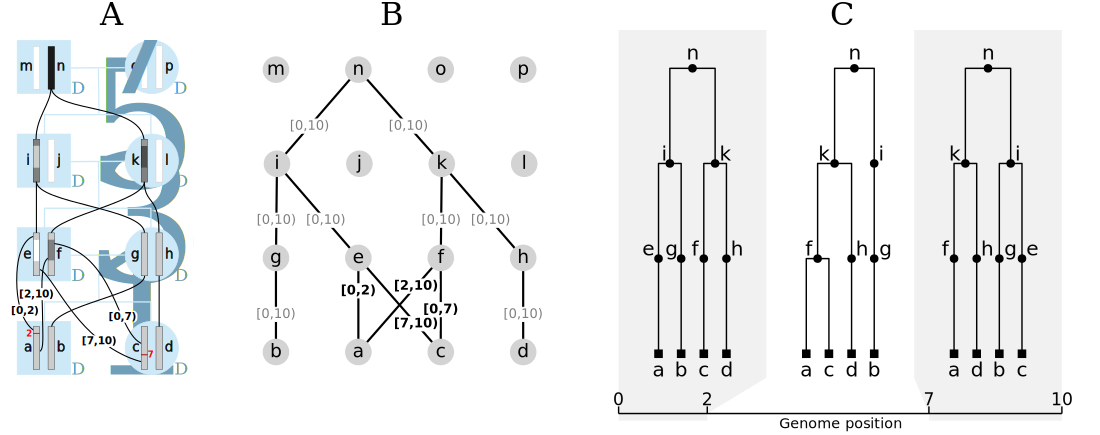
\includegraphics[width=0.75\textwidth]{illustrations/arg-in-pedigree}
\end{center}
\caption{\label{fig-arg-in-pedigree}
% TODO caption needs another pass. One the full section has been written
% it'll be clearer what we need to say in the caption vs the text.
[FIXME Update fig to make wider and less tall, and change $I$ to $D$.
Also possibly add some tabular encoding of gARG data.]
An example genome ARG embedded in a pedigree.
(A) Diploid individuals, visualised in a highly inbred pedigree and
labelled $D_1$ to $D_8$,
contain both paternal and maternal  genomes
labelled \textsf{a} to \textsf{p}. Black lines show inheritance paths connecting
genomes in the current generation (\textsf{a} to \textsf{d}) with their ancestors.
Genomes \textsf{a} and \textsf{c} are the product of two independent
recombination events between
the paternal genomes \textsf{e}
and \textsf{f}, and regions of genome inherited are shown.
Genomes are shaded such that where, backwards in time,
they merge into a common ancestor, the merged region is darker.
(B) The corresponding gARG along with inheritance annotations on all edges
(partial inheritance in bold).
(C) The corresponding local trees.
}
\end{figure}

As illustrated in Fig.~\ref{fig-arg-in-pedigree},
the gARG for a given set of individuals is embedded in their pedigree.
In this diploid example, each genome is inherited from one
of the individual's parents,
and may be the recombined product of that parent's two genomes.
For example, diploid individual $D_1$ in Fig.~\ref{fig-arg-in-pedigree}
has two genomes \noderef{a} and \noderef{b},
inherited from parents $D_3$ and $D_4$.
Genome \noderef{b} was inherited directly from $D_4$'s genome \noderef{g} without
recombination, whereas
\noderef{a} is the recombinant product of
$D_2$'s two genomes \noderef{e} and \noderef{f} crossing over at position 2.
This recombination means \noderef{a} inherits the (half-closed) genome
interval $[0, 2)$ from \noderef{e} and $[2, 10)$ from \noderef{f}.
These intervals are shown attached to the corresponding graph edges.


There are some important consequences to these definitions.
Firstly, there is
no limitation on mating system, ploidy, or age structure in a gARG.
By making the
basic unit of analysis an individual's genomes,
any pattern of inheritance among mixed ploidy (e.g.\ haplodiploid
species) can be accommodated.
Secondly, because we record the intervals of inheritance
between genomes,
arbitrary patterns of genetic inheritance such as
gene conversions,
multiple simultaneous recombinations
and so on can be directly expressed.
% Wilder: give forward ref to section on efficiency here, mention tree sequence
Thirdly, local trees that we generate for a particular position on the
genome can have nodes of any arity (number of child nodes), including ``unary''
nodes with a single child (see Section XXX).
% TODO should rephrase this from parent/child to ancestor/descendant?
Fourth, recombination is modelled in terms of
its outcomes in terms of inheritance intervals among parental genomes;
thus we will have a child node (the recombinant; e.g.\ node \noderef{a}
Fig.~\ref{fig-arg-in-pedigree}) and two (or more; see section XXX)
paternal genomes from which this child has inherited segments.
% TODO rephrase the above, it'll confuse people. Just need to reiterate the
% points about events, and maybe lead into the next section
Finally, gARGs are not defined in terms of the
coalescent with recombination (or any other) stochastic process.
Thus, the gARG encoding is focused on faithfully representing the
\emph{outcome} of the evolutionary processes of genetic inheritance
with recombination,
and is agnostic to the details of those processes.
% The paragraph above is a bit weak and muddled, needs a few more passes.
% In particular, the "Finally" bit doesn't really seem to follow
% from the others. Is there a more direct way we can address these points ?

% Firstly, a gARG may contain nodes that are both samples \emph{and}
% internal nodes in the local trees.
% This ability is useful when we have pedigree information
% along with genetic data
% \cite[e.g.][]{hayes20191000,RosFreixedes2022,anderson2022genes},
% where we may have many generations of internal sample nodes
% whose genomes have been sequenced.
% Another situation in which it is important that
% we do not assume samples are all contemporary ``leaf'' nodes
% (or that all internal nodes are either coalescences or recombinations)
% is when we are incorporating ancient genomes into ARG
% inference~\citep{speidel2021inferring,wohns2022unified}.
% Similarly, a gARG may contain nodes that
% do not correspond to any particular event in the ancestry of the samples.
% For example, node \textsf{h} is the direct ancestor of \textsf{d} in
% Fig~\ref{fig-arg-in-pedigree}, and is not the product of either a
% coalescence or a recombination. Such nodes would usually be removed
% from the graph so that \textsf{d} descends directly from \textsf{k} (see
% the ``\nameref{ARG_simplification}'' section) but there is no necessity for this from
% a representational perspective.
% Secondly, because we do not classify nodes by event type
% (common ancestor or recombination) there is no limitation
% on the complexity that can be modelled---multiple recombinations
% and coalescences can happen simultaneously in the same genome,
% a common occurance in large deeply sequenced
% pedigrees~\citep{hayes20191000,RosFreixedes2022}.
% Finally, there is a subtle and important point about how recombination
% is represented: which genome in the organismal lifecycle
% do nodes represent?
% In principle, we can interpret nodes as representing genomes
% at any point in the life cycle [supplementary Figure ?]. Hudson
% views nodes as representing gametes~\citep{hudson1983properties}.
% However, we argue that the most intuitive
% approach is to let nodes represent the genomes present in diploid
% individuals in each generation, as in
% Fig~\ref{fig-arg-in-pedigree}A. In this case recombination
% is not represented by a single ``recombination node'' (as in an eARG), but with
% two parent genomes between which recombination takes place
% (e.g.\ nodes \textsf{e} and \textsf{f}), and a
% single resulting ``recombinant'' genome (e.g.\ \textsf{c}). The
% edges that link this recombinant with its two parents carry the information
% concerning breakpoint location that would be associated with a
% recombination node in an eARG. [TODO finish up here with more
% clarity on what this means in terms of the required specifity
% of recombination events, and put in a forward ref to the simplification
% section where we talk about stacking up recombination events
% and their identifiability.]


\section*{Event ARGs}\label{eARG}
Genome ARGs are composed by
describing the details of genetic inheritance
between specific ancestor and descendant genomes.
In contrast, ARGs are classically defined
by the evolutionary \emph{events} in the history of a sample.
The difference between gARGs and this prevalent view of
what defines an ARG is subtle and difficult to distinguish.
It is therefore useful to first survey some representative
recent definitions of
an ARG from the literature, to allow us to capture their common features
(see Appendix XXX for a full review).

\citet{brandt2021evaluation} follow the original Griffiths definition of
an ARG by coupling it directly to a generative process, stating
that the ``full ancestral recombination graph (ARG) is a structure that encodes all
coalescence and recombination events resulting from the stochastic process of
the coalescent with recombination.''
\citet{shipilina2023origin} emphasise the true existence of the
corresponding events (rather than the generative process) by saying that
``[t]he ARG describes the complete
ancestry of a sample of genomes through a series of real coalescence and
recombination events.''
\cite{mathieson2020ancestry}
define an ARG as ``a subset of the pedigree...
contain[ing] only those edges along which inherited segments of DNA have been
transmitted, and only those nodes corresponding to ancestors in which there was
a recombination or coalescence event.''
% In contrast, ~\citet{gusfield2014recombinatorics} defines an ARG as [TODO]
% Papers that do not discuss how positions work:
% - Mathieson and Scally: no discussion of how it works concretely (but quite
%   close to gARG, in some ways)
% TODO list out some of these as examples of where people don't bother
% getting into this important detail?

The common feature of these definitions is that they are expressed
in terms of evolutionary \emph{events}, and so for the purposes of
discussion we can label
this prevailing interpretation as an ``Event ARG'', or eARG.
(Many definitions also emphasise
the necessity of exhaustively capturing \emph{all} events, which we
examine in later sections.)
Another common feature of these definitions is that they do not explicitly
discuss the mechanism by which genealogical trees vary along the genome.
The topology of an eARG defines the common ancestor and
recombination events that occured,
but the graph structure alone is not sufficient to define the local trees,
or equivalently, how ``ancestral material'' (Section XXX) flows along
the edges of the ARG.
This is usually assumed to follow the mechanism described by
Griffiths and colleagues in which we have
two different ``types'' of node in the graph:
common ancestor nodes in which the inbound lineages are merged into a
single ancestral lineage with one parent, and recombination
nodes in which a single lineage is split into two independent
ancestral lineages.
Recombination nodes are then
annotated with
the corresponding crossover breakpoint~\citep{griffiths1996ancestral}.
Fig.~\ref{fig-arg-data-structure} shows an example of a classical
eARG with three samples (\noderef{a}, \noderef{b}, and \noderef{c})
and a single recombination event, along with an example concrete
encoding of the data.  There is a single recombination event
at node \noderef{d} with a breakpoint at position $x$. We
assume that \noderef{d} inherits genetic material to the
left of $x$ from \noderef{e} and to the right of $x$ from \noderef{f}.
As shown in Fig.~\ref{fig-arg-data-structure}B,
the local trees are embedded in the graph, and can be reconstructed
in essentially the same manner as outlined the previous section for
gARGs. The only difference is that decisions about which outbound
edge to follow during the rootward traversal are taken at recombination
nodes, following
either the common convention that the order of parents
is significant~\citep[e.g.][]{griffiths1991two},
or by incorporating additional information to
distinguish left and right parents
into the
encoding~\citep[e.g.][]{gusfield2014recombinatorics,ignatieva2021kwarg}.

\begin{figure}
\centering
\tikzmath{\x1 =0; \x2=8;\xx=12.5; \x3=14; \xt=18;}
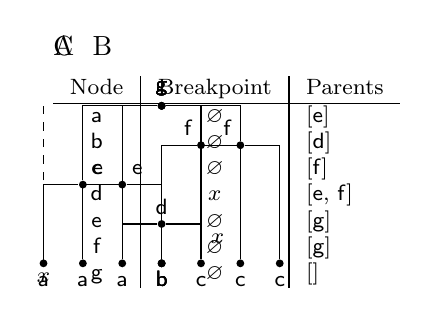
\begin{tikzpicture}[x=5mm, y=5mm, node distance=2mm and 20mm]
\tikzset{greynode/.style={circle,fill,inner sep=1},
nodelabel/.style={font=\footnotesize}}


\node [anchor=north west] at (\x1,6) {A};
\node [anchor=north west] at (\x2,6) {B};
\node [anchor=north west] at (\xt,6) {C};

%%% (A) ARG

\node (s0) [greynode] at (\x1 + 0, 0) {};
\node (s1) [greynode] at (\x1 + 3, 0) {};
\node (s2) [greynode] at (\x1 + 6, 0) {};
\node (s3) [greynode] at (\x1 + 3, 1) {};
\node (s4) [greynode] at (\x1 + 1, 2) {};
\node (s5) [greynode] at (\x1 + 5, 3) {};
\node (s6) [greynode] at (\x1 + 3, 4) {};

\draw (s1) -- (s3);
\draw (s0) |- (s4);
\draw (s4) -- (\x1 + 2,2) |- (s3);
\draw (s4) |- (s6);
\draw (s3) -- (\x1 + 4,1) |- (s5);
\draw (s2) |- (s5);
\draw (s5) |- (s6);

%%% (B) Trees
\node (l0) [greynode] at (\x2 + 0, 0) {};
\node (l1) [greynode] at (\x2 + 2, 0) {};
\node (l2) [greynode] at (\x2 + 3, 0) {};
\node (l3) [greynode] at (\x2 + 1, 2) {};
\node (l4) [greynode] at (\x2 + 2, 4) {};

\draw (l0) |- (l3);
\draw (l1) |- (l3);
\draw (l2) |- (l4);
\draw (l3) |- (l4);

\node (r0) [greynode] at (\x3 + 0, 0) {};
\node (r1) [greynode] at (\x3 + 1, 0) {};
\node (r2) [greynode] at (\x3 + 3, 0) {};
\node (r3) [greynode] at (\x3 + 2, 3) {};
\node (r4) [greynode] at (\x3 + 1, 4) {};

\draw (r0) |- (r4);
\draw (r1) |- (r3);
\draw (r2) |- (r3);
\draw (r3) |- (r4);

\foreach \u/\lab in {
        s0/$\textsf{a}$, s1/$\textsf{b}$, s2/$\textsf{c}$,
        r0/$\textsf{a}$, r1/$\textsf{b}$, r2/$\textsf{c}$,
        l0/$\textsf{a}$, l1/$\textsf{b}$, l2/$\textsf{c}$}
    \node[nodelabel,anchor=south] at ([yshift=-12pt]\u) {\lab};

\foreach \u/\lab in {
        s6/$\textsf{g}$,
        l4/$\textsf{g}$,
        r4/$\textsf{g}$}
    \node[nodelabel,anchor=south] at (\u) {\lab};

\node [nodelabel,anchor=north west] at ($(s3) + (\x1 + 0,0)$) {$x$};
\foreach \u/\lab in {
        s4/$\textsf{e}$,
        l3/$\textsf{e}$}
    \node[nodelabel,anchor=south west] at (\u) {\lab};
\foreach \u/\lab in {
        s5/$\textsf{f}$,
        r3/$\textsf{f}$}
    \node[nodelabel,anchor=south east] at (\u) {\lab};
\foreach \u/\lab in {s3/$\textsf{d}$, s6/$\textsf{g}$}
    \node[nodelabel,anchor=south] at (\u) {\lab};

\draw[dashed] (\xx,0) -- (\xx, 4);
\node[nodelabel,anchor=north] at (\xx,0) {$x$};


%%% (C) Encoding
\node [nodelabel,anchor=north west] at ($(\xt,5)$) {
\begin{tabular}{c|c|l}
% \multicolumn{2}{c}{Breakpoints}\\
Node & Breakpoint & Parents\\
\hline
$\noderef{a}$ & $\varnothing$ & [\noderef{e}]\\
$\noderef{b}$ & $\varnothing$ & [\noderef{d}] \\
$\noderef{c}$ & $\varnothing$ & [\noderef{f}]\\
$\noderef{d}$ & $x$ & [\noderef{e}, \noderef{f}] \\
$\noderef{e}$ & $\varnothing$ & [\noderef{g}]\\
$\noderef{f}$ & $\varnothing$ & [\noderef{g}]\\
$\noderef{g}$ & $\varnothing$ & []\\
\end{tabular}};

\end{tikzpicture}
\caption{\label{fig-arg-data-structure}
A classical event ARG. (A) Standard graph depiction with
breakpoint $x$ associated with the recombination node \noderef{d}.
Nodes \noderef{e}, \noderef{f} and \noderef{g} are common ancestor events.
(B) Corresponding local trees to the left and right of breakpoint $x$
(note these are shown in the conventional form in which only coalescences
within the local tree are included; see section XXX for a discussion
of this important point).
(C) A concrete encoding of the information (right).
Recombination nodes have a non-null breakpoint
and two parents.
}
\end{figure}

Whether we regard nodes as events or genomes is something of a
philosophical question, and in most senses the two are equivalent
(but see the discussion on ``unary nodes'' in section XXX).
From a concrete data-structure encoding perspective, the only real
difference between an eARG and a gARG is that we store recombination
\emph{breakpoints} at nodes of out-degree two (recombination nodes)
in an eARG and we store \emph{inheritance intervals} on the edges
of a gARG. A key advantage of associating inheritance intervals with
edges in a gARG is that it allows us to describe evolutionary events other
than simple crossovers, such as multiple recombinations and
gene-conversions. By explicitly stating the exact regions of genome
that are transmitted along an edge, we generalise the representation
to encompass any process that leads to the differential inheritance of
genetic material along the genome.

While the additional generality provided by the gARG representation
is useful, it is in reality a small change that does not
lead to significantly different time or space complexity in computational
tasks.
The vitally important and fundamental distinction between
a gARG and an eARG is that gARGs
allow us to directly describe
genetic inheritance in multiple non-contiguous genome intervals
between an ancestor and a descendant, which cannot be done
by specifying recombination events and breakpoints.
% FIXME this sentence is problematic. We should recast to talk about
% the outcomes of events, not talk about simulateousness (which will
% confuse people
Thus, we have the means of encoding the \emph{effects} of
multiple evolutionary events, and to
systematically describe the uncertainty around their
ordering (see Section XXX).
As we see in the following sections, freeing ourselves from the requirement
of recording specific events and
the additional generality of the gARG encoding
has many advantages. It also raises questions about what our goals
for inferring ARGs should be, and how we evaluate the success
of such inferences.

\section*{Prospective vs retrospective ARGs}
Event ARGs, as defined in the previous section as a way of encompassing
the range of definitions provided in the literature, are
inherently \emph{retrospective}.
Event ARGs are defined in terms
of the events that occur in the history of some set of sampled
sequences.
For example, Fig.~\ref{fig-arg-in-pedigree}
is retrospective because it only includes information
about genetic inheritance relative to the sample individuals
$D_1$ and $D_2$ (genomes \textsf{a}--\textsf{d}).
That is, only the inheritance
history of the sample genomes is recorded in the ARG.
% Gregor & Jerome think that "inheritance" is clearer here than "transmission"
Genetic inheritance must have occurred between (e.g.)
$D_8$ and her daughter $D_6$, but this is not recorded because
it is not relevant to the genetic ancestry of the sample

Genome ARGs, on the hand,
can be either retrospective or \emph{prospective}.
The edges in a gARG represent a path of genetic inheritance from
ancestor to descendant through some
% Wilder: finds the cell-to-cell confusing. Maybe drop?
number of generations (ultimately from cell to cell),
and are annotated
with the genome coordinates over which inheritance occurs.
In a prospective gARG, the inheritance intervals $I$
on an edge joining ancestor genome $v$ and descendant $u$
defines \emph{all} regions of genome that $u$ inherited from $v$.
Thus, these  inheritance intervals are
concerned only with the genetic relationship
between the nodes in question, and are not defined with respect
to any given set of samples. We are simply recording the
genetic inheritance between two genomes
(in the simplest case, between a parent and a child).

Prospective ARGs arise in individual-based forwards-time
simulations~\citep{kelleher2018efficient,haller2018tree},
where the genetic inheritance between genomes is recorded
exhaustively and periodically
``simplified'' to retain only
the ancestry relevant to the current population.
\citet{kelleher2018efficient} refer to the structure
recording all such forwards-in-time genetic relationships
as an ``embellished pedigree`` (and suggest the term ``nedigree'' as a shorthand).
Describing this instead as a ``prospective ARG'', emphasising
the use of the same data structures and the direct connection with
the usual retrospective interpretation of an ARG, may be
more useful.
The ``simplify'' algorithm, which prunes away parts of the graph that
are not ancestral to a sample, is the key enabling factor for
this approach to forwards-time simulation and is
described in detail by
\citet{kelleher2018efficient}.
It is a powerful tool for simulation and analysis, as it
allows to efficiently subset ARGs both in terms of the
samples and levels of detail about recombination retained,
as we discuss in the following sections.

\section*{Converting an eARG to a gARG}
Any eARG can be converted to a gARG without loss of information,
and the conversion process is very similar to
simplifying a prospective gARG with respect to a set of samples.
The process involves two steps, and is illustrated in
Fig.~\ref{fig-ancestry-resolution}.
The first step is straightforward (Fig.~\ref{fig-ancestry-resolution}B):
we duplicate the nodes and
edges from the input eARG, and then add inheritance annotations
to the output gARG's edges. If the node is a common ancestor node,
we annotate the single outbound edge with the interval $[0,L)$,
for a genome of length $L$.
If the node is a recombination event with a breakpoint $x$,
we annotate the two outbound edges with the intervals $[0, x)$
and $[x, L)$, respectively.
These inheritance annotations are clearly in one-to-one
correspondance with the information in the input eARG,
but they are a superset of the
``ancestral material''~\citep{wiuf1999ancestry,wiuf1999recombination}
of the sample.


\begin{figure}
\centering
% TODO update the source of this figure to make less tall. It's taking
% up far too much vspace at in native coords at the moment.
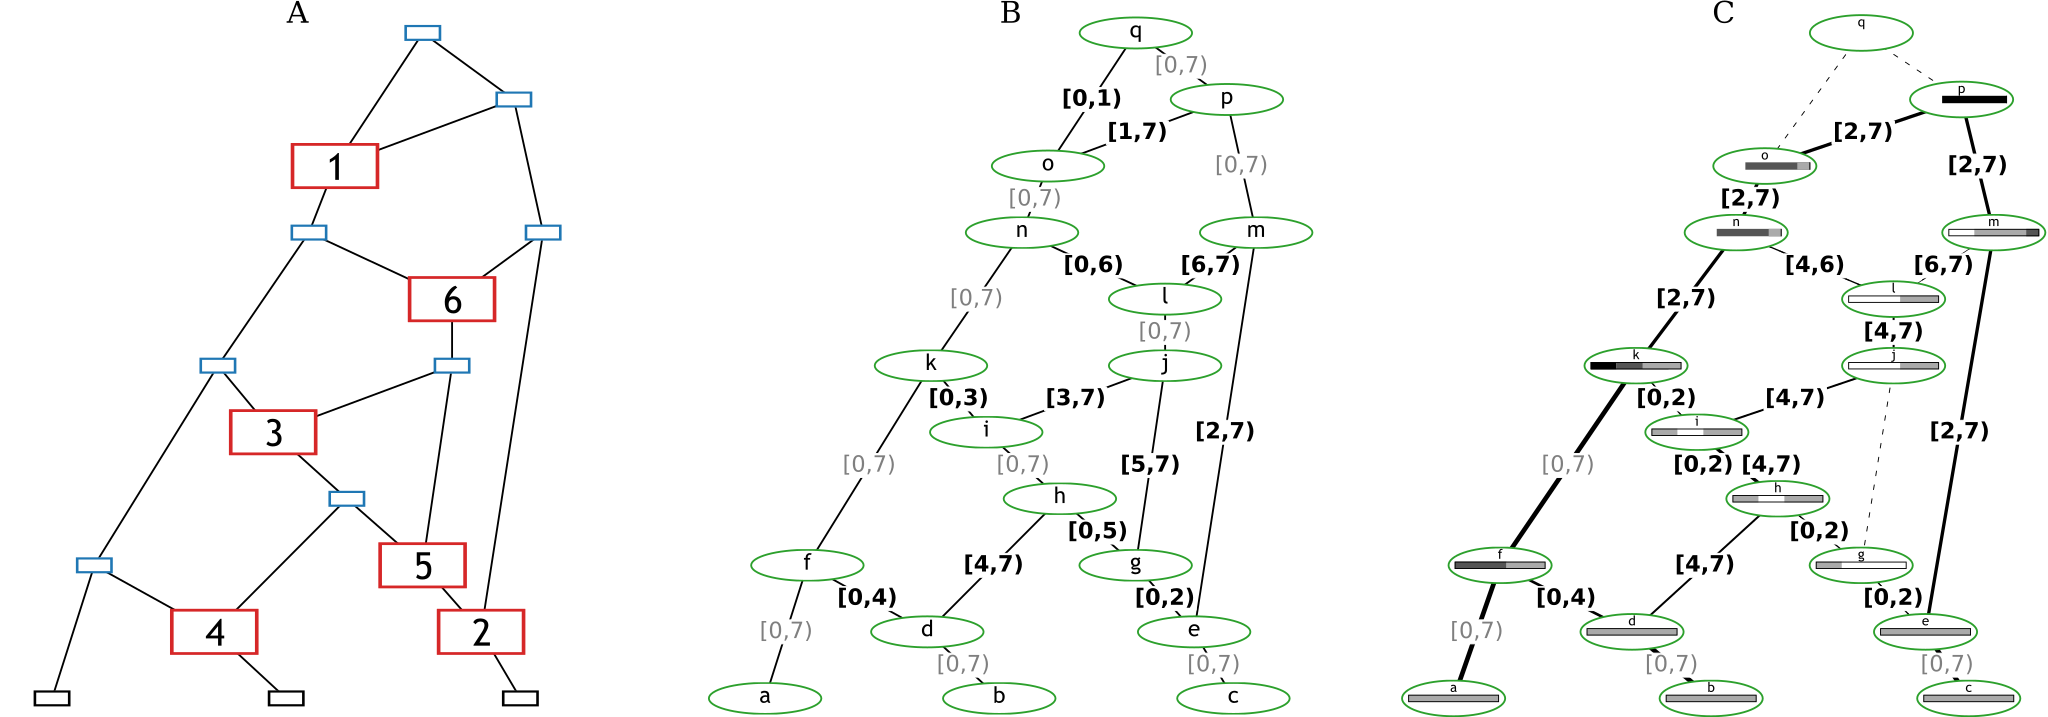
\includegraphics[width=\textwidth]{illustrations/ancestry-resolution}
\caption{\label{fig-ancestry-resolution}
Converting the \citet[][Fig.~1]{wiuf1999recombination} example
to a gARG. (A) The original eARG; square nodes represent events, with
each recombination (red) containing a breakpoint.
(B) The corresponding gARG with breakpoints directly converted to
edges annotated with inheritance intervals.
(C) The sample-resolved gARG resulting from simplifying with respect
to the samples, \noderef{a}, \noderef{b}, and \noderef{c}.
Dashed lines show edges that are
no longer present (in practice, nodes \noderef{g}, \noderef{j}, and \noderef{q} would also be removed).
Coalescence with respect to the sample is indicated by shaded bars, as
in Fig~\ref{fig-arg-in-pedigree}A; nodes \noderef{n}, \noderef{o}, \noderef{p}, \noderef{q} have incomplete
bars showing that local ancestry of entirely coalesced regions is omitted.
Line thickness is proportional to the genomic span of each edge.
Nodes representing recombination events are retained
for clarity, but could be removed by simplification if
desired.
}
\end{figure}

Ancestral material is a critical concept in a retrospective ARG,
and refers to the genomic intervals ancestral to the samples
scattered across lineages (the edges of the graph)
at some time in the past. At recombination
events, ancestral material is split between the ancestral lineages.
As genome segments coalesce in a common
ancestor the total amount of ancestral material is reduced, until
eventually, as we traverse rootwards through the graph, all
samples reach a most recent common ancestor at every location
along the genome. The process of transmitting ancestral material
along the edges of an ARG is directly analogous to Hudson's
simulation algorithm for the coalescent with
recombination~\citep{hudson1983testing,kelleher2016efficient}.

Fig.~\ref{fig-ancestry-resolution}C shows the graph that we obtain
by resolving the ancestral material transmitted along each edge
using the ``simplify'' algorithm~\citep{kelleher2018efficient},
and highlights some important
differences between the eARG and gARG encodings.
Firstly, we can see that some nodes and edges are removed entirely
from the graph by this conversion process.
The ``grand MRCA'' \noderef{q} is omitted from the
sample resolved gARG because all segments of the genome have
fully coalesced before it is reached. Likewise, the edge
between \noderef{g} and \noderef{j} is omitted because the recombination
event at position $5$ (represented by node \noderef{g})
fell in non-ancestral material.
More generally, we can see that the sample resolved
retrospective gARG of Fig.~\ref{fig-ancestry-resolution}C
allows for ``local'' inspection
of an ARG in a way that is not possible by storing
common ancestor and recombination events in an eARG. Because
the ancestral material is stored with each edge, the
cumulative effects of events over time can be reasoned
about, without first ``replaying'' those events. Many computations
that we wish to perform on an ARG will require resolving
the ancestral material with respect to a sample.
% this is weak, but would be good to emphasise this point.
% you just end up running simplify lots of times, in your
% downstream algs
The gARG encoding
allows us to do this once and to store the result, whereas
the eARG encoding requires us to repeat the process
each time.

Note that the \citet{wiuf1999recombination} eARG
in Fig.~\ref{fig-ancestry-resolution} is not particularly
representative, because inference or simulation methods will usually
only generate ARGs containing nodes and edges ancestral to the sample
(see the discussion of the ``Big ARG'' stochastic process in Appendix XXX, however).
Nonetheless, it is an instructive example from the literature which highlights several
important properties of ARGs, and the general point about
the need to resolve ancestral material ``on the fly'' for eARG traversals
holds.

\section*{ARGs and local trees}
Local trees, describing the genetic genealogy of a sample
at a particular location along the genome, are
embedded within in ARG, and the relationship
between the two is subtle and important.
% An ARG is sometimes referred to as being equivalent to a set of
% local trees along the genome [TODO citation], but the connection
% between the two is subtle.
% In order for the mapping to be one-to-one, so that the original
% gARG can be exactly recovered from a set of local trees and
% their genome coordinates,
% some specific properties of the ARG and the trees are required.
Note that many authors use the term ``marginal''
trees~\citep[e.g.][]{griffiths1996ancestral,minichiello2006mapping} [more]
which we avoid due the potential confusion with the
statistical concept of marginal distributions
(which could lead to interpretation as an integrated tree over many positions).

It is useful to have
a concrete definition and explicit process for local tree extraction.
We can describe a local tree as an
oriented tree~\cite[p.\ 461]{knuth11combinatorial},
a sequence of integers $\pi_1\pi_2\dots$ where $\pi_u$ denotes the parent of
node $u$~\citep{kelleher2013coalescent,kelleher2014coalescent,kelleher2016efficient}.
If $u$ is a root
% I'm not sure if this reachability stuff is a helpful clarification, and whether it'll just
% confuse people. It depends on some tricky details.
(or not reachable from the samples)
in the local tree at position $x$, then $\pi_u = -1$ (by convention).
% JK: this confused some people, so best left out?
% Technically, this structure is a ``forest'', as it allows us to have
% multiple disconnected trees, which occurs when all samples have not
% found a most recent common ancestor.
Oriented trees allow nodes
to have  any number of children; from one (see section XXX for more
discussion on such ``unary nodes'' in the local trees), to arbitrarily
large polytomies.
To recover the local tree $\pi$ at position $x$, we begin by
setting $\pi_u = -1$ for each $u\in N$. Then, for each sample
node in $S$ we trace its path rootwards through the
ARG for position $x$, and record this path in $\pi$.
Specifically, at a given node $u$,
we an find edge $(c, p, I) \in E$ such that $u = c$ and $x \in I$, and set
$\pi_c \leftarrow p$. We then set $u \leftarrow p$, and repeat
until either $\pi_u \neq -1$ (indicating we have traversed this section
of the ARG already on the path from another sample) or there
is no matching outbound edge (indicating we are at a root).

The nodes in a local tree encoded
in this way are \emph{labelled} (i.e.\ carry the identity
of the corresponding ARG node), and this is fundamentally
important to how a local tree relates to its parent ARG.
If we are given the sequence of local trees for a gARG
encoded as an oriented tree (or in any other form in which
the tree nodes are explicitly labelled with the identity of the
corresponding ARG node)
along with the genome interval covered by each tree,
then we can recover precisely the same ARG. Thus, there
is a one-to-one correspondance between an ARG and
the sequence of local trees that it encodes.

The internal nodes of trees, however, are usually
considered to be \emph{unlabelled},
because they most often correspond
to anonymous hypothetical ancestors.
Internal ARG nodes likewise correspond to anonymous hypothetical
ancestors, but if we do not label them we lose the fact that
the \emph{same} ancestors persist across multiple trees.
Without labelled internal tree nodes,
we must infer their identity
from the tree topology, which is both
expensive to compute and imprecise. For example
we could infer that node \textsf{k} is shared in the second
and third trees of in Fig.~\ref{fig-simplification}D
because it subtends identical subtrees in both,
but it would not be straightforward to infer that it
is also the root of the first tree.

\cite{shipilina2023origin} discuss the same ideas,
and note that the
``full ARG ... contains more information than the series of tree
sequences along the genome''.
Their statement that an ARG
contains more information than its local trees is true only if
the local trees are unlabeled and/or do not contain unary nodes.
However, as we have shown, if the local trees
contain labelled internal (possibly unary) nodes,
then  there is precisely as
much information in them as an ARG.
Whether such unary nodes are \emph{observable}
is an entirely separate question, of course.

These properties have interesting consequences when we
consider the inference strategy of estimating local trees
independently and subsequently stitching them together
into an ARG.
Two recent methods take this approach,
\relate~\citep{speidel2019method} and
\espalier~\citep{rasmussen2022espalier},
and have different strategies for reconciling the local trees into an ARG.
\relate\ first infers local tree topologies, and then identifies
edges that persist from tree to tree by reasoning about the sets of samples
subtended. It does not attempt to be exhaustive.
\espalier, on the other hand, is specifically interested
in the details of recombination events (among small samples)
and therefore attempts to infer
the precise subtree prune-and-regraft (SPR)
operations~\citep{hein1990reconstructing,song2003on,song2006properties}
induced by recombination.
Inferring the SPRs between leaf-labelled trees is
NP-hard~\citep{hein1996complexity,allen2001subtree,bordewich2005computational},
but it is unclear what the complexity is when there
is a degree of internal node sharing between trees.


% The equivalence between an ARG and a set of local trees
% separated by SPRs is often mentioned [e.g. x y z], but
% it is important to note that while extracting local
% trees from an ARG is straightforward, the converse
% process of reconstructing precisely the same ARG from
% these trees is more problematic. If the internal
% nodes are consistently labelled and unary nodes are
% included in the local trees (e.g., Fig~\ref{fig-simplification})
% then it is easy to exactly reconstruct the ARG.
% Otherwise, the problem is much more difficult and it
% may not be possible to uniquely reconstruct the original ARG.
% Without labels for the internal nodes, we are forced to
% to reason about which subtrees remain the same and which
% differ due to the SPR separating adjacent trees in order to
% assign node identity. Without the internal unary nodes marking
% recombinations, we must infer their existence. In
% general, there will not be a unique solution to this problem,
% and so there can be many possible ARGs compatible with
% a given list of leaf-labelled binary trees.
% This is the approach taken by the Espalier inference
% method~\citep{rasmussen2022espalier}, which finds a
% set of SPRs that reconcile independently inferred
% trees from different regions of the genome.


\section*{Levels of simplification}\label{ARG_simplification}
ARG simplification is a powerful tool, and can do much more
besides removing unreachable nodes and edges in a prospective ARG
and resolving ancestral material in an eARG.
In general, we can think of
ARG simplification as the process
of removing nodes and re-writing edges (and their inheritance annotations)
to remove various types of redundancy.
The redundancy that we are interested in
revolves around the presence of nodes that appear
``unary'' in one or more local trees
(where a node has exactly one child over a particular genomic region).
These arise in several different ways.
Nodes with one child are not a standard feature of evolutionary trees;
we are usually interested in
nodes that have at least two children, because these
are in principle detectable from mutational differences
arising in the respective subtrees.
A tree branch may correspond to many generations
of individuals
% Following feedback from Wilder, this is more likely to confuse
% people unless we properly explain
% (or indeed cell divisions)
and there is usually
very little information about these intermediates, or utility
in modelling them.
% FIXME the bridge between the next few paragraphs is a bit weird, in
% that we've just been talking about how interesting unary nodes are
% but then go on about how to remove them. Just needs a bit of smoothing
% out I think.
ARGs, however, are different, and there
can be significant information about evolutionary processes
provided by nodes that are unary in one or more local trees.
% Not sure what to do with this - should mention though.
\citet{mathieson2020ancestry} show examples in which the ARGs
contain unary nodes, and state that paths are
``implicitly passing through points representing specific individuals.''
% Full quote from fig caption:
% Genetic ancestry in the form of the ARG for a single individual. Combining
% genetic ancestry from different positions leads to a graph, incorporating all
% realized genetic ancestry paths, implicitly passing through points representing
% specific individuals.

\begin{figure}
\centering
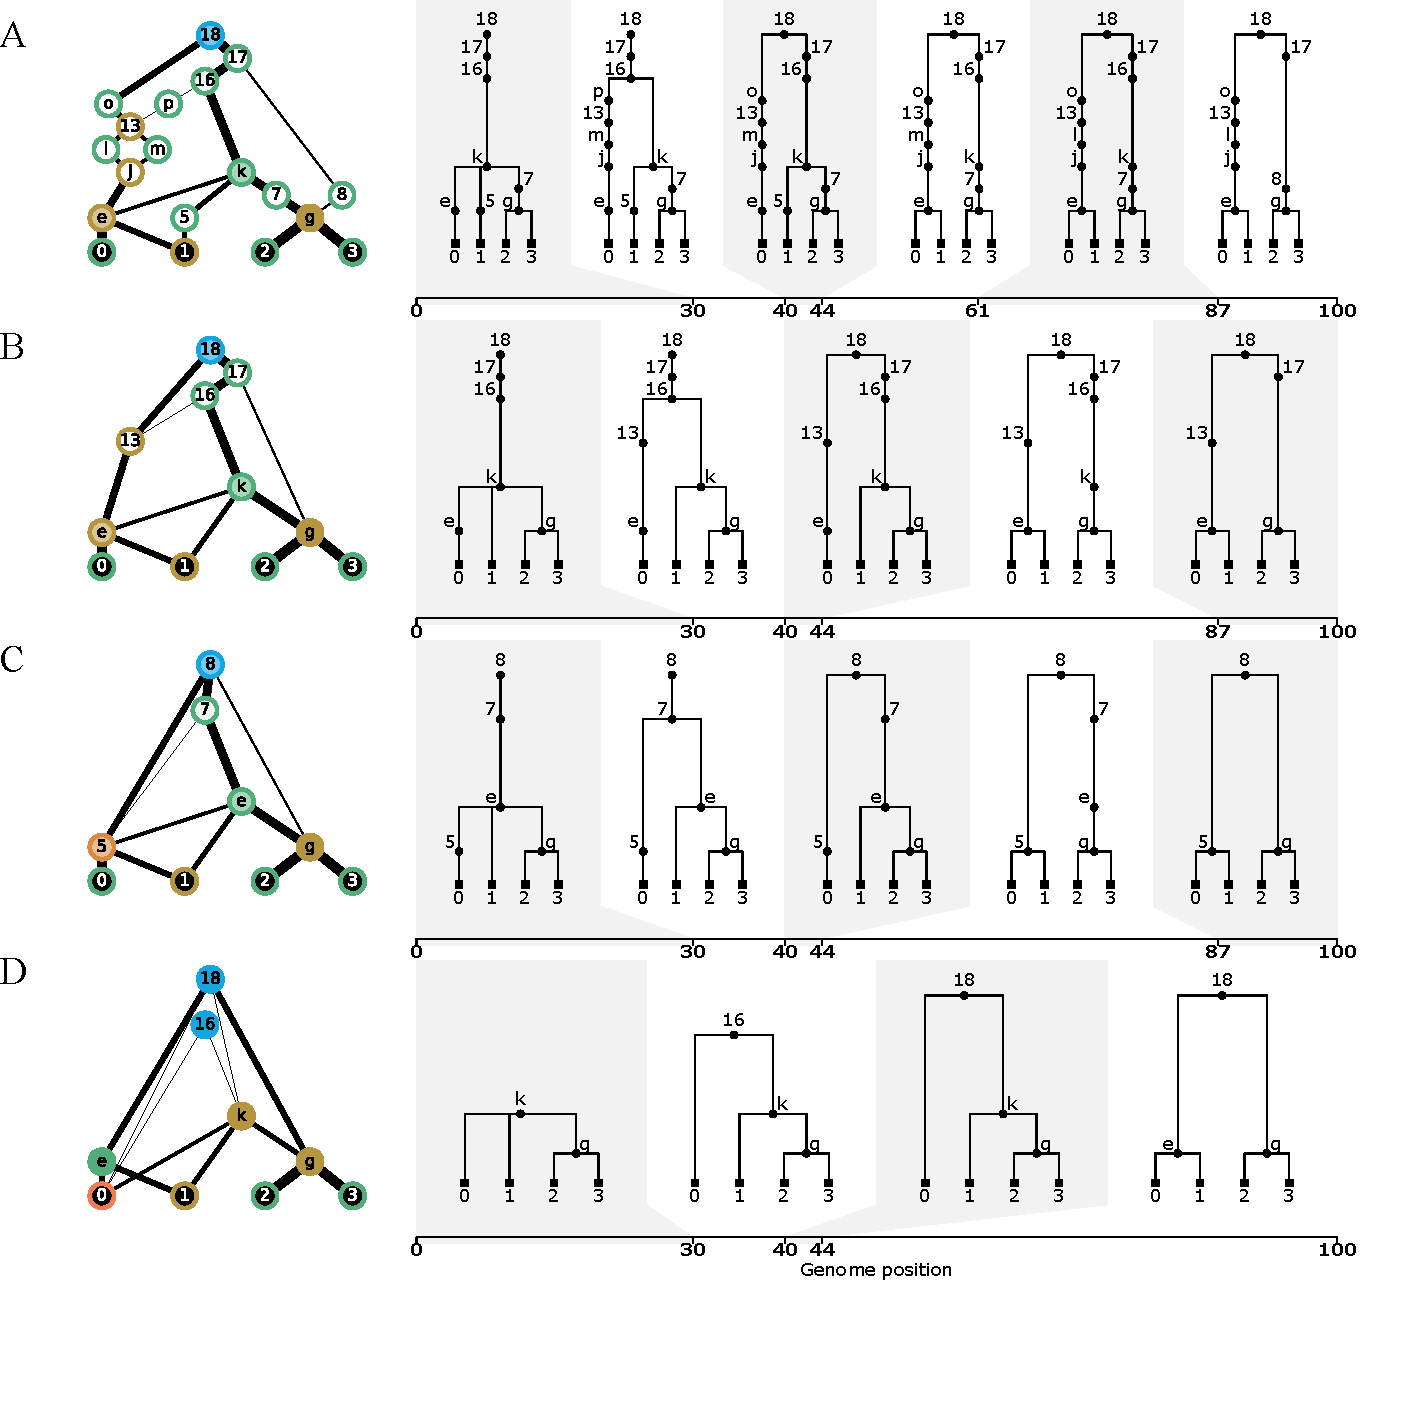
\includegraphics[width=\textwidth]{illustrations/simplification}
\caption{\label{fig-simplification}
Levels of ARG simplification.
In all cases the graph visualization is shown on the left
and the corresponding local trees on the right.
Nodes are coloured by the number of parents and shaded
according to the proportion of their span over which they are coalescent.
(A) A gARG simulated from a backward-time diploid Wright-Fisher
model: genome \noderef{k} has three children, and the genomes
\noderef{e} and \noderef{g} simultaneously have multiple parents and multiple children.
(B) Simplified to remove all
singly-connected graph components (e.g., diamonds such as \noderef{jlnm}).
(C) Remove nodes that never represent coalescences,
i.e.\ are unary everywhere (e.g.\ \noderef{n} and \noderef{r}).
(D) Rewrite edges to bypass any unary nodes in local trees.
}
\end{figure}

Fig.~\ref{fig-simplification} shows a series of successive steps of
simplification,
% FIXME this doesn't explain anything - what did we store in the simulation?
starting with a sample-resolved but unsimplified gARG, simulated under a
backward-time Wright-Fisher
model. We show the graph on the left, and the corresponding sequence of
local trees on the right.
In Fig.~\ref{fig-simplification}A the local trees (right)
contain many unary nodes, and as we successively simplify,
the local trees contain fewer
unary nodes (Fig.~\ref{fig-simplification}B,C) until
we reach Fig.~\ref{fig-simplification}D, where the local trees
have no unary nodes.
A node is unary in a local tree covering the genome interval $I$
if genetic inheritance passes through that ARG node,
but no coalescence occurs in the interval $I$.
The distinction between the ``common ancestry'' of two or more genomes
in an ancestral genome and the ``coalescence'' which may or may
not occur in the local trees is
important~\citep{hudson1983testing,kelleher2016efficient}.
Consider \noderef{e} in Fig.~\ref{fig-simplification}A,
for example. We can see from the graph that it is a common
ancestor of  samples \noderef{a} and \noderef{b}, but
it does not correspond to any coalescence in the
local trees to the left of position $44$, and is therefore
unary in these three trees.

The first level of simplification that we can perform is to remove
graph topology that is invisible to the samples.
An example of such topology is a
``diamond''~\citep{rasmussen2014genome}
in which the two parent nodes of a recombination immediately
join again into a common ancestor (e.g.~\noderef{j}, \noderef{l}, \noderef{m}
and \noderef{n} in Fig.~\ref{fig-simplification}A).
Unless we are specifically
interested in the recombination event or these ancestral genomes,
there is no information in this topology and the diamond can be
replaced by a single edge. More generally, any
subgraph that is singly-connected in both the leafward and
rootward direction (a ``super-diamond'') is non-identifiable and can be
replaced by one edge. This definition includes the case
of a node that has one inbound and one outbound edge, such as
nodes \noderef{f} and \noderef{h}.
Fig.~\ref{fig-simplification}B shows the result of this type of
graph topology simplification.

Simplifying away diamonds will remove many unary nodes from the
local trees, but there can still be nodes that are unary in all
of the local trees. In particular, a node can represent a recombinant
with multiple parents in the graph but only a single child (e.g.\ node \noderef{n}
in Fig.~\ref{fig-simplification}B), or can represent a common ancestor with
multiple children in the graph but in which no coalescence takes place
in the local trees
(node \noderef{r} in Fig.~\ref{fig-simplification}B).
% point out that this is why Hudson refers to CA nodes, not coalescence nodes
Such nodes are not singly connected in the graph, but are nevertheless unary in
all of the local trees.
The operation to remove them
therefore requires knowledge not just of the graph topology but also of the
ancestral material associated with the edges.
As we see in Fig.~\ref{fig-simplification}C,
removal of recombinant nodes can produce graph nodes with
more than two parents (e.g.~node \noderef{e}); and likewise, removal of
common ancestor but non-coalescent nodes can produce graph nodes with
more than two children (e.g.~node \noderef{s}). These represent a ``stacking up'' of
the \emph{effects} of multiple evolutionary events in a single node (genome), and the
ARG no longer contains the intermediate genomes representing those events.

% JK: Text moved from an earlier section. See if we want to reuse this here
% if not already said.
% Indeed a single node can have both multiple children
% and multiple parents. This would be the case in Fig~\ref{fig-arg-in-pedigree} if,
% for instance, node \noderef{a} were to have two children.
% % It is a shame that this is not actually shown in fig 3, but I don't think
% % we can do this unless we have 5 generations
% Moreover, a single node can have more than 2 children, and (as we shall see in
% the ``\nameref{ARG_simplification}'' section), more than 2 parents. Another way to
% state this is that transitions between nodes in a gARG can encapsulate multiple
% events in an eARG.

The remaining nodes are MRCAs of some subset of the samples
at \emph{some} positions along the genome. We still have
some unary nodes in the local trees, but these nodes will
correspond to a coalescence in at least one other
local tree. For example, node  \noderef{k} is unary in the fourth tree
of Fig.~\ref{fig-simplification}C, but is either binary
or ternary in all other local trees (recall this is a Wright-Fisher
simulation). The final level of simplification is to alter the edge annotations
such that, although no nodes are removed from the graph, all
unary nodes disappear from the local trees (Fig.~\ref{fig-simplification}D).
Note that although this last stage produces simpler local trees, by
removing information about the exact paths taken by lineages through
the graph, we lose potentially useful information about shared edges
between trees. The extent to which this information can be inferred
and utilised is an interesting open question.
% I don't think there's an actual manuscript or title to refer to here
% [CITE Ralph in prep.].

An important consequence of simplifying ARGs to remove
unary nodes in local trees is that we lose some information
about recombination
events. This is related to the amount of \emph{precision} about
recombination events that we store, which is the topic of the next
section.

\section*{Precision of recombination information}
\label{sec-precision}
% The ARGs in Fig.~\ref{fig-simplification} represent different
% levels of detail about the same ancestral history. They represent
% the same set of recombination and common ancestor events,
As illustrated in Fig.~\ref{fig-simplification}, successive levels
of ARG simplification reduce the amount of information about the
history of the sample that is stored. Some of the information lost,
e.g.\ ``diamond'' removal (Fig.~\ref{fig-simplification}A),
seems like a reasonable tradeoff for a simpler structure.
The consequences of other simplifications, however, are
more subtle and relate directly to what can be known about
recombination events and the levels of precision that
we should seek to infer about them.

The ARGs in Fig.~\ref{fig-simplification} contain different
numbers of local trees ($6$, $5$, $5$ and $4$ for A through
D, respectively). When we move from A to B the local trees
for the intervals $[44,61)$ and $[61,87)$ are merged because
the only differences between them are their paths through
nodes \noderef{l} and \noderef{m}. These nodes that participated
in the diamond are removed from the ARG, and we have lost
all information about the corresponding recombination at
position 61. Other nodes (e.g.\ \noderef{o} and \noderef{p})
have also been removed but these represent the \emph{parents}
of recombinants. The recombinant nodes themselves
(e.g. \noderef{n}) are still present, and represent precise
information about the time, genomic location and tree
branches involved
in the recombination event.

Fig.~\ref{fig-simplification}C has the same number of local trees
as Fig.~\ref{fig-simplification}B, but has less precise information
about recombination. Continuing the previous example, node
\noderef{n} has been removed from the graph because it was unary
in all of the local trees; its outbound edges to \noderef{s}
and \noderef{q} have effectively been ``pushed down''
to \noderef{e} (which is retained because it is the coalescent
parent of \noderef{a} and \noderef{b} over the interval
$[44, 100)$). We
have therefore lost precision about
the \emph{timing} of this recombination event, and know only
that it must have occured between the times of node \noderef{e}
and \noderef{q}.

Fig.~\ref{fig-simplification}D removes all unary nodes from the
local trees, and further reduces the precision of
recombination information. Node \noderef{e} has not been
removed from the graph because it is coalescent in the
final tree, but we no longer know that the recombination
event at position 30 was ancestral to it, or have
any indication of its timings. Furthermore,
trees for $[44, 87)$ and $[87, 100)$ were only distinguishable
by the passage of the former tree through nodes \noderef{e}
and \noderef{q}, and so the recombination on node \noderef{g}
at position 87 has been lost entirely.

% The point of these examples is to emphasise that
% information about recombination in an ARG is not ``all
% or nothing'': there is a gradation of detail
% about recombination, in terms of genomic location, timing,
% and the ancestral lineages involved.
% While there has been a recent tendancy to emphasise the
% importance of ``full ARGs''
% \citep[e.g.][]{deng2021distribution,brandt2021evaluation,
% rasmussen2022espalier}
% which contain complete information about all recombination
% events, it is reasonable to question the value of
% such precise information and whether it is knowable.
% [SOME MORE STUFF]

% Ancestral recombination graphs are often characterised
% as consisting of a complete record of the genetic history
% of a sample. For example,
% \cite{rasmussen2014genome} state that an ``ARG provides a record of all
% coalescence and recombination events since the divergence of the sequences
% under study'' and
% according to \cite{deng2021distribution} an ARG
% ``provides all the information about the genealogical history of a sample,
% including the locations of recombination events.'' It is worth
% questioning, however, whether such comprehensive information
% will always be available, and in particular whether our
% representation of genealogical history should \emph{require}
% such precision. Simulations will usually generate complete
% information about the history of a sample, of course, but
% we may not have sufficient information to infer such detail.

% % The full ancestral recombination graph (ARG) is a structure that encodes all
% % coalescence and recombination events resulting from the stochastic process of
% % the coalescent with recombination.
% \citet{brandt2021evaluation} define a ``full'' ARG as
% ``a structure that encodes all
% coalescence and recombination events resulting from the stochastic process of
% the coalescent with recombination'' (thus going against the general
% historial trend discussed in the XXX section).
% \citet{rasmussen2022espalier} have a less restrictive definition, in
% which a ``full'' ARG is one that contains complete information about
% recombination events, without necessarily being tied to a particular
% stochastic process.
% While [something positive], it is important to be clear on
% what the overall goal of such precise inferences are,
% what the limitations on when they can be made are,
% and their downstream utility in applications.

% % What is the goal of having fully precise ARGs?
% % 1) studying the actual recombination events;
% % 2) evaluating the likelihoods
% The main reasons for wanting precise estimates of all recombination
% events are to either compute a likelihood of the inferred ARG
% under a statistical model, or to study the recombinants in
% detail~\citep{rasmussen2022espalier}.
% % Explain that we're really interested in the details of recombination
% % itself with a small number of samples.
% In the latter case, we might
% have a small number of samples~\citep{guo2022recombination}.

% Beyond cases in which visual inspection of the trees and the
% effects of recombination is feasible, the main application
% of having completely precise estimates of recombination events is
% to evaluate the likelihood of the estimate under some
% statistical model. The only statistical model available
% is the coalescent with recombination
% and its approximations~\citep{mcvean2005approximating,marjoram2006fast}.
% In this case, the utility of a ``full`` ARG for some dataset
% is limited by how well the dataset fits the assumptions
% of the model.

% % JK: This is very rough, just jotting down the basic ideas,
% % will need substantial revision.
% It is not clear that such complete information will always
% (or indeed ever) be available from inferences~\cite{shipilina2023origin}.
%  We may be
% able to precisely identify the location and timing
% of recent recombinations (particularly if detailed pedigree
% information is available) but beyond this, the information
% required simply isn't present. When sampling from a
% process such as the Sequentially Markov
% Coalescent~\citep{mcvean2005approximating,marjoram2006fast}
% like ARGweaver~\citep{rasmussen2014genome}, it is true that
% we do obtain a fully resolved ARG with precise
% information about recombination, but it is reasonable
% to question how much information from the data is used
% to support older recombinations, in particular.

% % This idea of a continuum of information about recombination
% % being inferrable and representable is consistent with the ideas
% % discussed by~\cite{shipilina2023origin}. There a haplotype block
% % is synonymous with coalescent nodes in the ARG, which we can generalise
% % as nodes in a gARG with at least two children. In principle, these
% % nodes are identifiable by the mutations that occur on the outbound
% % edges of the node.

% It is helpful to consider the difference between fully
% resolved binary trees and those that contain polytomies.
% The situation is in fact directly analogous: an ARG that
% contains fully resolved recombination information must have
% at two most parents per node.

% In general, discussions tend to contrast an ARG
% on one hand as holding \emph{complete} information about recombination
% (and therefore between-tree correlation structure)
% and a sequence of local trees on the other (with, by implication,
% no direct information about between-tree correlations).
% This is a false dichotomy:
% a \emph{continuum} of information about recombination and between-tree
% correlation structure can be represented and inferred, and all
% such levels of information are useful, even if only for computational
% efficiency.

\begin{figure} \begin{center}
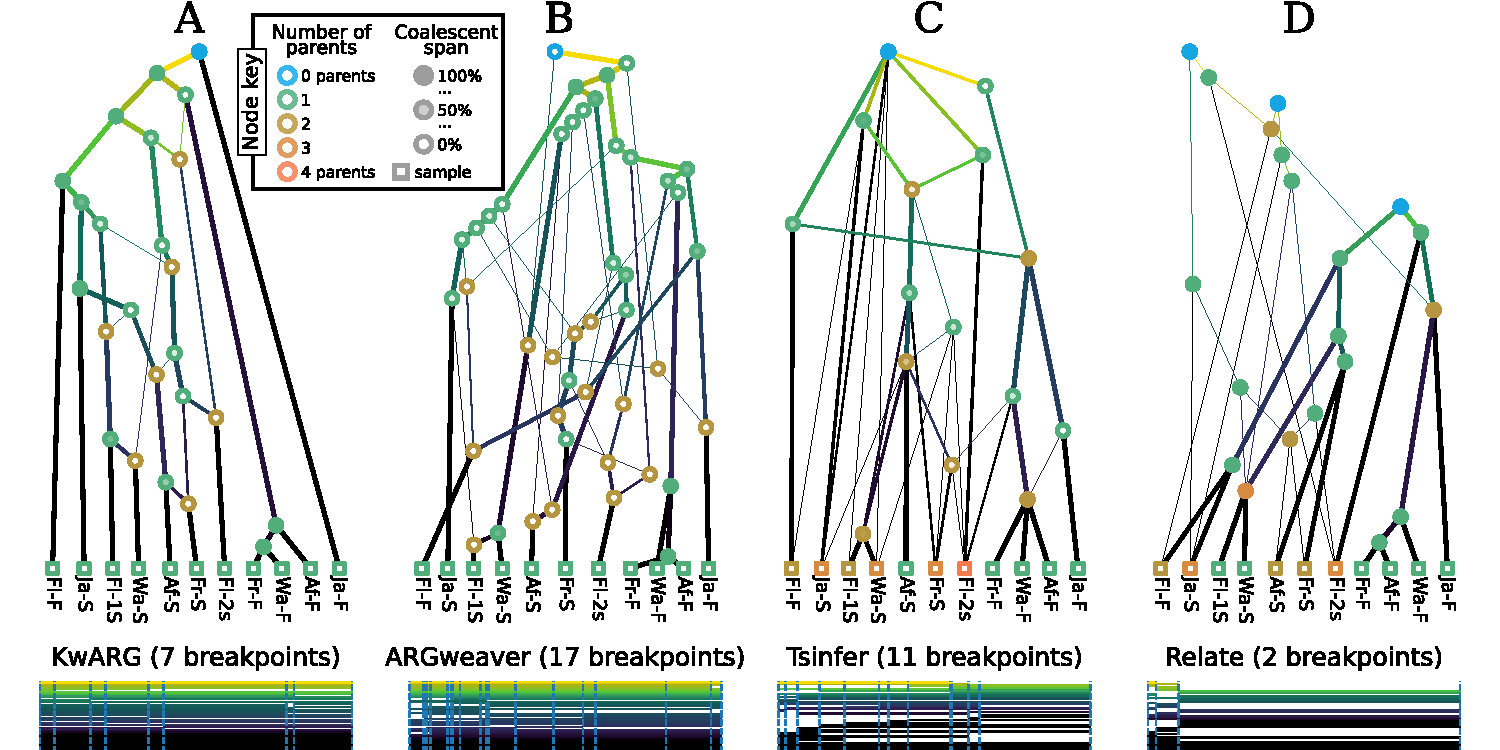
\includegraphics[width=\textwidth]{illustrations/inference.pdf} \end{center}
\caption{\label{fig-inferred-args} Inference results for
(A) \kwarg, (B) \argweaver, (C) \tsinfer,
and (D) \relate\
for 11 samples of a 2.7kb region of the \textit{Drosophila melanogaster} ADH
locus~\citep{kreitman1983nucleotide}.
The \argweaver\ example
is a sample from the inferred posterior distribution.
Edge colours are based on the time of the edge's child node
(lighter: older; darker: younger).
Line width corresponds to the genomic span of the edge.
Position on the X and Y axes for the graph visualization is arbitrary.
 Node colour
refers to the number of parents of the node.
The fill colour intensity of a node is determined by the genomic span over which
it has two or more children divided by the span where it has any
children (the ``coalescent span'').
The genomic intervals associated with edges are shown below
each ARG, where each row is an edge
and the X axis reflects genomic position.
Vertical lines indicate breakpoints between local trees.
}
\end{figure}

The example of successive simplification of a simulated ARG
in Fig.~\ref{fig-simplification} illustrates the point
that is is possible to \emph{store} arbitrary levels of precision
about recombination in a gARG.
It is also possible to \emph{infer} various levels of precision about
recombination.
To illustrate this, and to demonstrate the structural
heterogeneity of the ARGs inferred  by current methods,
Fig.~\ref{fig-inferred-args} shows the results ARG inference
% To illustrate these points and to emphasise the heterogeneity
% of the ARGs inferred by current methods, we inferred ARGs for the
for the classical \citet{kreitman1983nucleotide} benchmark dataset
using  \kwarg~\citep{ignatieva2021kwarg},
\argweaver~\citep{rasmussen2014genome,hubisz2020inference},
\tsinfer~\citep{kelleher2019inferring},
and \relate~\citep{speidel2019method}.
% While there is some consistency among the inferred ARGs (such as the samples
% FR-F, WA-F and Af-F being grouped into the same clade), there
% are also considerable differences.
The minimum number
of recombination breakpoints required in the absence of recurrent mutation
is 7 for this dataset~\citep{song2003parsimonious},
and the number of inferred breakpoints
under the input mutation and recombination rates
varies from 2 (\relate) to 17 (\argweaver).
% TODO this needs a bit of rewriting with the rest of the paper in mind
% kwarg and argweaver are inferring eARGs, but we need to be careful
% not to confuse people.
The ARGs inferred by the different methods also have major differences
in how recombination information is represented.
Essentially,
\kwarg\ and \argweaver\ infer eARGs that contain
specific causal recombination \emph{events} for each breakpoint.
On the other hand, \tsinfer\ and
\relate\ do not infer causal events but rather
infer gARGs with differing levels of precision about recombination.
The bottom row of Fig~\ref{fig-inferred-args} shows the extent along
the genome to which graph edges are shared between multiple trees.
We can see, for example, that the \relate\ trees ``share'' less topology
than other methods, but it certainly does not infer a series of
\emph{unrelated} local trees (i.e., with either unlabelled internal
nodes or differently labelled nodes in each tree).
The ARGs inferred by \relate\ and \tsinfer\ both contain substantial
information about node sharing across trees; for example,
both infer that Af-f, Fr-f and Wa-f share a common ancestor along
the entire sequence.
They contain a level of detail about recombination
that lies somewhere between a sequence of unrelated local trees on one
extreme and a completely precise event ARG on the other.

\section*{Computational efficiency and data interchange}
ARG inference methods have been successfully applied to vast datasets,
including 500,000 genotyped humans~\citep{kelleher2019inferring,zhang2023biobank}
from UK Biobank~\citep{bycroft2018genome}
and over a million SARS-Cov-2 whole genomes~\citep{zhan2023towards}.
Even larger datasets are
available~\citep[e.g.][]{halldorsson2022sequences} % TODO more
and it seems inevitable that ARGs will be inferred for them.
The efficiency with which we can store and analyse these inferred
ARGs is therefore of great importantance, and a key factor
in the ultimate success of downstream ARG-based methods.
Another key factor in how important ARG-based methods become
across the wide range of predicted application
% TODO more?
areas~\citep{rasmussen2014genome,harris2019database,
hejase2020summary,schaefer2021ancestral,
fan2022genealogical,wohns2022unified,harris2023using,
nowbandegani2023extremely}
is how well inference methods and downstream analysis applications
interoperate. Without a well-defined and efficient shared format
for ARG data interchange,
users will suffer from problems of converting data from one programs
output to another, an unfortunate hallmark of population genetics
software for many years~\citep{excoffier2006computer}.
While current methods tend to tightly couple downstream analysis
of the inferred ARG with the inference
itself within the same software package,
this approach scales poorly in terms of software development
effort, and is ultimately not compatible with the widespread use
of ARGs for routine data analysis, and a healthy and diverse
software ecosystem.

The gARG encoding discussed and concretely defined in this manuscript
leads to highly efficient storage and processing of ARG data,
and has already been in use for several years.
The succinct tree sequence data structure (usually known as a ``tree sequence''
for brevity)
is a concrete encoding of a gARG, as discussed in this article.
It was originally developed as part of the \texttt{msprime}
simulator~\citep{kelleher2016efficient} and subsequently been
extended and applied to forward-time
simulations~\citep{kelleher2018efficient,haller2018tree},
inference from data~\citep{kelleher2019inferring,wohns2022unified},
and calculation of population genetics statistics~\citep{ralph2020efficiently}.
The succinct tree sequence encoding extends the basic definition
of a gARG provided here by stipulating a
simple tabular representation and nodes and edges,
and also defining a concise and lossless representation of
sequence variation using the ``site'' and  ``mutation'' tables.
(Technically, edges in tree sequence terminology would be better
described as ``edge-intervals'', as each describes a single continguous
interval of genome inheritance between a pair of nodes. This
denormalisation of the gARG data model is for efficiency purposes.)
The \texttt{tskit} library is a liberally
licensed open source toolkit that provides a comprehensive suite
of tools for working with gARGs (encoded as a succinct tree sequence).
Based on core functionality written
in C, it provides interfaces in C, Python and Rust.
Tskit is mature software, widely used in population genetics, and
has been incorporated into several downstream
applications~\citep[e.g.,][]{haller2019slim,speidel2019method,
adrion2020community,
terasaki2021geonomics,
baumdicker2021efficient,
fan2022genealogical,korfmann2022weak,
mahmoudi2022bayesian,petr2022slendr,rasmussen2022espalier,
zhang2023biobank,nowbandegani2023extremely}.

% FIXME this needs more work and doesn't really fit into the
% narrative right now, but we do need to make this point.
The key insight that makes the succinct tree sequence encoding
an efficient substrate for defining analysis algorithms is that
it allows us to generate the local trees along the genome
in a way that allows us to reason about the \emph{differences}
between those trees.
Sequentially generating the local trees along the genome
is also fundamental, and is necessary whenever we need to
perform calculations that are contingent on more than just the
isolated properties of an edge. \cite{kelleher2016efficient}
showed how all trees can be sequentially generated in
constant time per tree transition in a fully simplified gARG.
Furthermore, we can easily reason about how tree topologies
change (and stay the same), leading to efficient algorithms
for computing population genetic
statistics~\citep{kelleher2016efficient,ralph2020efficiently},
implementing the Li and Stephens
model~\citep{kelleher2019inferring,wohns2022unified}
and likely many more.


%%%% Some old text about the coalescent we might still want to plunder
% % If we want to use the coalescent, then really the assumptions
% % need to make sense.
% % n << Ne is a silly assumption in today's datasets
% A core assumption of the coalescent is that the sample size $n$
% is much less than the effective population size, $N_e$.
% Several human datasets now consist of hundreds of thousands of
% genomes~\citep{bycroft2018genome,karczewski2020mutational,tanjo2021practical},
% and so sample size is substantially \emph{larger} than $N_e$
% (often assumed to be $10^4$ in humans).
% Agricultural datasets are even more extreme.
% For example,
% the US dairy cattle database alone currently comprises more than 6 million
% animals with SNP array
% genotypes\footnote{\url{https://queries.uscdcb.com/Genotype/counts.html}},
% while the effective population size in modern dairy cattle breeds is
% less than 100 and decreasing~\citep{MacLeod2013,Makanjuola2020}.
% An extreme sign of these breeding practices is that there are only two ancestral
% Y-chromosome lineages present in today's US Holstein dairy breed~\citep{Yue2015}.
% Simlarly, the 1000 bull genomes project~\citep{hayes20191000}
% comprises close to 7000 genomes, which are part of multi-generation pedigrees
% with millions of animals and extensive SNP array genotype and phenotype
% data \citep[e.g.][]{Cesarani2022}.
% In another example, genome and SNP array data for 440,610 individuals within
% 7 multi-generation pedigrees~\citep{whalen2018,Johnsson2021,Ros-Freixedes2020}
% were combined to infer recombination in pigs~\citep{RosFreixedes2022}.
% Effective population size in modern pig breeds is also less than 100 due to
% intense selection and directed reproduction \citep{Hall2016,Porcnic2016}.
% Another core assumption of the coalescent model is that the genome (or
% at least the region under study) is short enough that the number of extant
% lineages remains much smaller than $N_e$ at all times. Whole
% genome sequences have been available for model organisms
% for over a decade now, % True? Citation?
% and indeed complete chromosome-level assemblies are possible
% in humans~\citep{miga2020telomere}.
% Projects are under way to obtain high-quality assemblies
% for all eukaryotic species in Britain and Ireland~\citep{darwin2022sequence}
% and ultimately worldwide~\citep{lewin2022earth}.

\section*{Discussion}
Recent breakthroughs have made ARG inference methods practical
at scale for the first time, and there has been a surge of interest
in inference methods, their evaluation and application.
The prospect of ARGs being used routinely in population
and statistical genetics applications is tantalising,
but in reality there is substantial work to be done to
enable this.
A necessary first step is a degree of terminological clarity.
As discussed in Appendix XXX, the term Ancestral Recombination
Graph has several
subtly different interpretations depending on context.
The trend to decouple ARGs from their origins as a stochastic
process and instead use the term as a more general representation of any
recombinant genetic ancestry seems most useful, which we have
tried to clarify and systematise here. Thus
we can think of an ARG as any structure that encodes the
reticulate genetic ancestry of a sample of colinear sequences under
the influence of recombination. The ``genome'' ARG encoding
made explicit here is one way we can concretely
define such recombinant ancestry, which we have shown is both
flexible and efficient.
The flexibility of the gARG encoding contrasts with the classical
``event'' ARG (eARG), which is more limited in what can be described, because of its origins in an idealised mathematical model.

Fully decoupling the general concept of an ARG from the coalescent
with recombination stochastic process is an important step.
While it has proven to be a useful and
robust
model~\citep{wakeley2012gene,bhaskar2014distortion,nelson2020accounting},
many modern datasets have properties that grossly
violate its assumptions.
For example, several human datasets now consist of hundreds of thousands of
% TODO cite GeL paper
genomes~\citep{bycroft2018genome,karczewski2020mutational,tanjo2021practical},
and so sample size is substantially \emph{larger} than the
usually assumed $N_e$ values.
Agricultural datasets are an even more extreme departure from coalescent
assumptions, with hundreds of thousands of samples embedded in
multi-generational pedigrees~\citep{hayes20191000,Ros-Freixedes2020}
and effective population sizes of 100 and even
less~\citep{MacLeod2013,Makanjuola2020,Hall2016,Porcnic2016}.
Even if sufficiently complex demographic models~\citep{gower2022demes}
encompassing hundreds of populations, explosive growth rates and
myriad interconnections of migration, were somehow estimated and
provided as input, ARGs sampled from
the coalescent cannot capture the complexities of realistic family structures. There are many species with sizeable to large number of progeny, making polytomies a necessary feature of local trees. Flexible ARG encoding should accommodate such cases.

Given that there is no single model that can capture the complexities
of modern datasets across species (and taxa; see discussion of SARS-CoV-2
below), we cannot rely on sampling from a distribution to capture
the uncertainty in our ARG estimates. Indeed, even if the coalescent
was a suitable model for datasets such as UKB and we had a means of
sampling from its distribution of ARGs at the scale of hundreds of thousands
of samples, we could only explore the tiniest corner of such an incompehensibly
large space of possibilities.
Therefore, it is important to systematically
describe and utilise uncertainty about ARG inference.
One approach, enabled by the gARG encoding described here,
is to use polytomies and stacked recombinations as direct topological
descriptions of uncertainty. Other methods to capture, for example,
uncertainty about node ages and breakpoint locations, is an important
aspect of future work.

Uncertainty is a central element of inference about recombination,
and, even with small samples, we can only expect to uniquely identify
lineages and breakpoints in special cases.
[summarise info inferable about recomb in few sentenances here?
Cite: \citep{myers2002detection,hayman2023recoverability}]
% This might be where we mention Fisher's junctions and IBD?
% https://github.com/tskit-dev/what-is-an-arg-paper/issues/121
The fact that the classical ``event'' ARG (eARG) encoding
\emph{requires} completely precise estimates about recombination
is therefore a fundamental limitation, and a central message
of this paper.

% % Do downstream applications actually make use of such full ARGs?
Besides the inherent limitations that exist on inferring fully
precise ARGs from data,
we should also consider the value that such precise estimates provide
to downstream applications.
To date, few downstream applications using estimated ARGs
make use of complete recombination information.
Most applications work by examining local trees independently.
For example, the \relate\ selection statistic~\citep{speidel2019method}
computes selection $p$-values by comparing the coalescence rates at various time points.
In their method
for estimating dispersal rates and the locations of genetic
ancestors,
\citep{osmond2021estimating} downsample trees along the genome
so that they can be regarded as approximately independent.
The SIA method for detecting selection~\citep{hejase2022deep}
encodes local trees as a set of lineage counts at discrete
time intervals, and uses these as feature for a
type of machine learning algorithm
that takes ``temporal'' correlations into account. Thus,
while SIA does use some of the information about local tree correlation,
clearly much of the detail about recombination
events in an ARG is lost.
The \texttt{tsdate} algorithm (and related naive estimator
of ancestral location) uses much more between-tree
information~\citep{wohns2022unified}, explicitly using the gARG
encoding to reason about ancestral nodes.
The main application for fully precise ARGs thus far has been
to compute a likelihood under the coalescent with
recombination~\citep[e.g.][]{kuhner2000maximum,mahmoudi2022bayesian},
which currently requires the details of all recombination
events to be known.

% Note: haven't said anything about the coalescent here. Do we need to?
The advantages of a model-free representation that naturally
incorporates uncertainty about the ordering of events in and ARG are well illustrated by the
ARGs inferred for SARS-CoV-2 by~\cite{zhan2023towards}.
The COVID-19 pandemic led to collection of whole-genome viral data
at unprecented scale. The GISAID database~\citep{shu2017gisaid}
holds over 15 million sequences as of [FIXME].
Recombination, while rare, is an important
factor in the evolution of
SARS-CoV-2~\citep{vaninsberghe2021recombinant,jackson2021generation,ignatieva2022ongoing}
with recombinants potentially gaining fitness by combining
mutations from deeply diverged lineages [cite].
\citet{zhan2023towards} inferred two large ARGs for SARS-CoV-2 based
on GISAID data, one containing 1.27 million sequences sampled up to
June 30, 2021 and the other (more sparsely sampled) consisting of
657K sequences sampled up to June 30, 2022.
Sequencing effort at the height of the pandemic produced
tens of thousands of sequences collected in a single day,
with hundreds being identical.
Polytomies are therefore and unescapable reality, and a
fully-resolved binary tree would clearly be false precision.
Because of longitudinal data collection, there is no
requirement that samples must be leaf nodes, and samples
will frequently descend from other (older) samples.
Unary nodes (a node in a local tree with exactly one child)
are also a common feature, when a sample is inferred to have
exactly one direct descendant.
Despite the abundance of data and the rarity of recombination,
the parental lineages cannot be precisely identified
in many cases. For example, many are inferred to have three
or more parental lineages (in agreement with the
analysis resulting in the Pango designation of the recombinant
lineage); in most cases, these will indicate two or more
independent recombination events.
Faithfully representing the uncertainty
around these events seems a more useful approach than
the arbitrary resolution which would be required,
if encoded as an eARG.

% An interesting property of the SARS-CoV-2 dataset is that
% it highlights the uncertainty in the genomic position of
% recombination breakpoints. [Some discussion about why
% we can never know where the breakpoint really happened, and
% some follow-up to note that this is even more acute in
% standard popgen datasets where we're thinking about ancient
% recombs].
% This is a limitation of the
% gARG encoding proposed here, which requires that we specify
% exact intervals of inheritance and therefore precise
% recombination breakpoints.
% An approach in which we can systematically reason about the
% uncertainty of inheritance intervals as they propogate
% through an ARG
% would be an interesting avenue for future research.

This view of ARGs,
decoupled from generative models and
without the hard requirement
of complete precision on all historical events, may clarify inference goals and improve
methods for evaluation.
In most cases,
the accuracy of ARG inference is evaluated by comparing some truth simulations
to the inferred ARGs by the pairwise comparison of local trees along the genome
using tree distance
metrics~\citep[e.g.][]{robinson1981comparison,kendall2016mapping}
as originally proposed by \citet{kuhner2015assessing}.
% While this provides valuable insights into the method's performance,
% it is not clear how well these tree distance metrics reflect
% performance on real data.
In comparing tree-by-tree along the genome, the effects of recombination
structure is incorporated in an indirect manner, and the tree
metrics assume unlabelled nodes, effectively discarding information
about node sharing between trees.
Tree distance metrics usually have $O(n^2)$ time complexity and therefore cannot be
applied to the very large sample sizes currently of interest.
A recent trend has been to move away from such tree distance-based approaches and to examine more properties of the inferred ARGs.
\citet{brandt2021evaluation} compared the
distributions of time to the most recent common ancestor across several
methods, which captures many important aspects of dated ARGs
but neglects [SOME OTHER THINGS].
\citet{deng2021distribution} derived the distribution of the expected
waiting distances to tree changes, and compared this to the
outputs of several methods.
[ \citet{ignatieva2023distribution} DID SOMETHING ELSE]
% Not sure this is the right place for this sentence
All of these evaluations have been based on
ground truth data from highly idealised simulations
with small sample sizes,
and the effects of the richness of real data
(beyond simplistic error models)
on modern biobank scale or multi-generational pedigree datasets
are almost entirely unknown.
A suite of true ARG evaluation metrics, that take into account more of the
global topology and can be applied to large ARGs, would be a
valuable addition to the field.

[TODO finish up with a positive note about interchange, and make the point
clearly that tskit is an ARG library. Splice in the stuff about haplotype
blocks and ARGON format here somewhere --- basically this is a derived product
of the gARG encoding, so while there are some computation advantages it's not
fundamental to the actual representation of the thing]

Earlier efforts to standardise ARG interchange
did not succeed~\citep{cardona2008extended,mcgill2013graphml}.

In summary, we advocate for decoupling between generative models that give rise to observed data and data formats that can faithfully and realistically encode these data. We have shown that ``genome'' ARG (gARG) encoding enables flexible encoding of today's datasets with realistic levels of precision. Importantly, genome ARG encoding should facilitate easier data interchange between different tools, which will in turn support active research in this area.

% \cite{shipilina2023origin} discuss the idea of a ``haplotype block''
% (equivalent to the ``bricked tree sequence'' of
% \cite{nowbandegani2023extremely},
% % TODO look this up. I expect it's basically the same??
% and the block-based ARG data structure of
% \citep{palamara2016argon}),
% here we consider the unique sets of
% samples that coalesce at a node in the ARG over a particular
% genome interval, and the fundamental limitations they place
% on ARG inference.
% [FIXME find somewhere natural for this. The last clause is too vague - what
% are the implications?]
% Alternative gARG encodings split transmitted intervals and associate each with
% a new node, resulting in a single genome being represented by a group of
% multiple nodes (or ``blocks'' \citep{palamara2016argon}), with implications for

\section*{Acknowledgements}
We are grateful to Gideon Bradburd and Alex Lewanski for helpful discussions
and comments on the manuscript.

\bibliographystyle{plainnat}
\bibliography{paper}

\setcounter{secnumdepth}{2} % Print out appendix section numbers

% TODO revisit number here
\section*{Appendix}
\appendix

\section{Ancestral graphs: a brief history}
\label{sec-arg-history}
The coalescent~\citep{kingman1982coalescent,kingman1982genealogy,
hudson1983testing, tajima1983evolutionary} models the ancestry of a sample of
genomes under an idealised population model, and provides the theoretical
underpinning for much of contemporary population genetics.
It is a stochastic process, where each random realisation
is a genealogical tree describing the genetic ancestry of the sample.
Numerous extensions to the model have been
proposed~\citep{hudson1990gene,hein2004gene,wakely2008coalescent},
incorporating many evolutionary processes.
\citet{hudson1983properties}
first incorporated recombination into the coalescent process,
providing several fundamental analytical results
and describing the basic simulation algorithm, still in
widespread use~\citep{hudson2002generating,kelleher2016efficient,
baumdicker2021efficient}.
In the 1990s, Griffiths and colleagues revisited the
coalescent with recombination from a different perspective,
formulating it as a stochastic process where each realisation
is encoded as a graph~\citep{griffiths1991two,ethier1990two,
griffiths1996ancestral,griffiths1997ancestral}.
They referred to both the stochastic process and
its random realisations as the Ancestral Recombination Graph (ARG).
Although mathematically equivalent, it is
important to note that the Griffiths and Hudson formulations of
the coalescent with recombination are not identical;
in particular, a direct implementation of the ARG process
as originally described requires exponential time to simulate
(see Appendix XXX for details). However, ARGs provided a way
to reason about and infer recombinant ancestry as a single object,
which was not possible within Hudson's framework, which emphasised
the collection of local trees along the genome resulting from recombination.

Subsequent work on ARGs proceeded in broadly three main directions: focussing on (1)
exploring the mathematical properties of the coalescent with recombination and
related stochastic processes, (2) inferring evolutionary parameters under
(approximations to) this model, either with or without explicitly reconstructing the
genealogy of the sample, and (3) treating the ARG as a discrete graph, ignoring the
generating stochastic process, and studying its properties from a computational and
algorithmic perspective.

% Mathematical treatment of the CwR and ARGs (and ARG-like stochastic processes)
An extensive body of work has been developed from
studying the coalescent with recombination
% Can we add a couple of the most well known CwR examples here
and other related
graph-valued stochastic processes from a mathematical perspective.
In particular, the Ancestral Selection Graph
(ASG)~\citep{krone1997ancestral,neuhauser1997genealogy}
uses a similar approach to model natural selection instead of recombination.
Unlike the ARG process, the ASG imposes a hard distinction between the stochastic process,
which constructs a random ARG-like graph, and an observable realisation,
which is a single tree sampled from the graph in a non-uniform way to encode
desired patterns of natural selection.
Constructions of ASG-like stochastic processes encoding various
forms of selection, often in parallel with recombination or other genetic forces,
are an area of considerable and ongoing theoretical interest~\citep[e.g.][]{
neuhauser1999ancestral,
donnelly1999genealogical,
fearnhead2001perfect,
fearnhead2003ancestral,
etheridge2009coalescent,
gonzalezcasanova2018duality,
koskela2019robust}.
% Could mention the Ancestral Gene Transfer graph here too, within
% something like "Similarly the Ancestral Gene Transfer Graph [cite]
% and [other ancestral graphs, if they exist?] model genealogical
% processes in bacteria as a graph.

% Inference of parameters and explicit ARG reconstruction
Early work on inference under the coalescent with recombination
focused on the problem of
inferring the parameters of the
stochastic process, where the ancestry was regarded as a
latent parameter to be averaged out
\citep[e.g.][]{griffiths1996ancestral,kuhner2000maximum, nielsen2000estimation,
fearnhead2001estimating}.
These methods met with limited success
because the state space of ARGs is overwhelmingly large, and
lacks a simple geometry or neighbourhood structure for inference or
sampling methods to  exploit.
Several breakthroughs in this direction were achieved through
formulating simplified but more tractable approximations to the full
model~\citep{mcvean2005approximating,marjoram2006fast,li2011inference,
paul2011accurate,schiffels2014inferring}.
The related problem of \emph{sampling} genealogies compatible with a given
dataset under the coalescent with recombination also proved notoriously difficult
computationally; progress in explicitly inferring genealogies at scale
has similarly been achieved through resorting to principled
approximations~\citep{rasmussen2014genome,mahmoudi2022bayesian},
or moving away from the coalescent with recombination altogether and seeking
to infer a single plausible ARG~\citep[e.g.][]{speidel2019method} or ARG
topology~\citep[e.g.][]{minichiello2006mapping,kelleher2019inferring}.

% Optimisation problems to do with ARGs and other phylogenetic networks
There has also been substantial interest in formulating and answering
fundamental questions about properties
of the ARG as a discrete graph structure, abstracting away from the
generating process and focussing on the ARG topology without considering
branch lengths.
The first prominent problem was calculating (lower bounds on) the minimum number of
recombinations required to reconstruct a valid genealogy for a given
sample~\citep{myers2003bounds}, and constructing the corresponding
minimal (parsimonious)
ARGs~\citep{song2003parsimonious,song2005efficient,lyngso2005minimum}.
These problems are NP-hard in general~\citep{wang2001perfect}, and progress has
been achieved through studying various constrained special cases of ARGs~\citep[e.g.][]{gusfield2004optimal} and
other more general types of phylogenetic networks~\citep{huson2010phylogenetic}. The
focus has been on algorithmic and combinatorial results, that largely do not
have direct relevance to the inference problems described above.

%It is important to note that parsimonious ARGs
%have quite different properties from realisations of the
%ARG \emph{process} as modelled by Hudson, Griffiths, and colleagues.
%Firstly, branch lengths are not typically estimated,
%% why do we need the following two lines
%and node times are required in order to compute a likelihood under the
%coalescent with recombination (see section XXX).
%Secondly, even if branch lengths were estimated,
%the realisations would have a very small likelihood since
%the coalescent with recombination is often highly \emph{un}parsimonious
%in terms of recombination events.

The goal of this historical overview is to illustrate that the meaning of the term ``ARG" now strongly
depends on the context in which it is used, and can mean both the
stochastic process generating genealogies in the presence of
recombination~\citep[e.g.][]{nordborg2000linkage,birkner2013ancestral,
wilton2015smc,griffiths2016coalescent},
as well as, more commonly, the concrete realisation of ancestry from a
process~\citep[e.g.][]{gusfield2014recombinatorics,mathieson2020ancestry,brandt2021evaluation}.
\cite{minichiello2006mapping} explicitly distinguished the ARG as a
stochastic process from the ARG as a data structure, and
argued for using the term to mean specific realised ancestral histories.
Unless otherwise stated, we will use the ARG-as-a-data-structure
interpretation for the remainder of this paper.

% FIXME putting this here for now just to see if this will work.

% \section*{Event ARGs}\label{eARG}
% In keeping with its original derivation in terms of a stochastic
% process (see Appendix~\ref{sec-arg-history}), the classical definition of an
% ARG data structure is
% in terms of events.
% Nodes represent
% common ancestor or recombination events that occurred in the
% history of some set of sample genomes, and edges represent ancestral
% lineages~\citep{griffiths1996ancestral}.
% In a common ancestor event the inbound lineages are merged into a
% single ancestral lineage, and in a recombination
% event a lineage is split into two independent
% ancestral lineages.
% % The final vital
% % detail is that we associate a breakpoint with each recombination
% % event.
% % This information is sufficient to uniquely
% % define the local genealogical trees at every position along the genome,
% % which is the basic requirement for a data structure encoding
% % genome-wide genetic ancestry.
% As illustrated in Fig.~\ref{fig-arg-data-structure}, this information
% is usually concretely encoded by associating a recombination breakpoint
% (which is null for common ancestor events) and an ordered list of parents
% with each node. We refer to such a  data structure as an
% ``event ARG'' (eARG).
% To recover the local tree at genome coordinate $x$ (the most
% fundamental operation required for an ARG data structure),
% we traverse the graph rootwards from the leaves.
% At a particular
% node $u$, if it has one parent we are at a common ancestor
% node and we follow that parent. If we are at a
% recombination node, $u$ has two parents: if
% $x$ is less than the breakpoint we follow
% the edge to the first parent, and otherwise follow the edge
% to the second parent.
% The order in which parents are listed at a recombination node is
% therefore significant, telling us
% from which parent the segments of genome to the left and right of the breakpoint
% were inherited.

% This ordering requirement, while straightforward
% to describe, has some practical drawbacks. For example,
% % Surely the meaning is clear from the context here and we don't need
% % qualify the meaning of ``ARG''
% when using this representation and simulating an ARG backwards in time,
% the first event older than a recombination may involve the lineage carrying the
% ancestry to the right of the breakpoint rather
% than the left, and so we cannot emit edges as they are generated.
% Such issues can be worked around, of course, but depending on the ordering of
% otherwise indistinguishable objects is generally problematic.

% \begin{figure}
% \centering
% % \begin{tabular}{cc}
% \begin{tikzpicture}[x=5mm, y=5mm, node distance=2mm and 20mm]
% \tikzset{greynode/.style={circle,fill,inner sep=1},
% nodelabel/.style={font=\footnotesize}}

% \node (s0) [greynode] at (0, 0) {};
% \node (s1) [greynode] at (3, 0) {};
% \node (s2) [greynode] at (6, 0) {};
% \node (s3) [greynode] at (3, 1) {};
% \node (s4) [greynode] at (1, 2) {};
% \node (s5) [greynode] at (5, 3) {};
% \node (s6) [greynode] at (3, 4) {};

% % \node [anchor=north west] at (0,6) {A};
% \node [nodelabel,anchor=north west] at ($(s3) + (0,0)$) {$x$};
% \foreach \u/\lab in {s0/$\textsf{a}$, s1/$\textsf{b}$, s2/$\textsf{c}$} \node[nodelabel,anchor=north] at (\u) {\lab};
% \foreach \u/\lab in {s4/$\textsf{e}$} \node[nodelabel,anchor=south west] at (\u) {\lab};
% \foreach \u/\lab in {s5/$\textsf{f}$} \node[nodelabel,anchor=south east] at (\u) {\lab};
% \foreach \u/\lab in {s3/$\textsf{d}$, s6/$\textsf{g}$} \node[nodelabel,anchor=south] at (\u) {\lab};

% %% Edges
% \draw (s1) -- (s3);
% \draw (s0) |- (s4);
% \draw (s4) -- (2,2) |- (s3);
% \draw (s4) |- (s6);
% \draw (s3) -- (4,1) |- (s5);
% \draw (s2) |- (s5);
% \draw (s5) |- (s6);

% % \node [anchor=north west] at (9,6) {B};
% \node [nodelabel,anchor=north west] at ($(10,5)$) {
% \begin{tabular}{c|c|l}
% % \multicolumn{2}{c}{Breakpoints}\\
% Node & Breakpoint & Parents\\
% \hline
% $\noderef{a}$ & $\varnothing$ & [\noderef{e}]\\
% $\noderef{b}$ & $\varnothing$ & [\noderef{d}] \\
% $\noderef{c}$ & $\varnothing$ & [\noderef{f}]\\
% $\noderef{d}$ & $x$ & [\noderef{e}, \noderef{f}] \\
% $\noderef{e}$ & $\varnothing$ & [\noderef{g}]\\
% $\noderef{f}$ & $\varnothing$ & [\noderef{g}]\\
% $\noderef{g}$ & $\varnothing$ & []\\
% \end{tabular}};


% % \node [anchor=north west] at (9,6) {C};
% % \node [nodelabel,anchor=north west] at ($(10,5)$) {
% % \begin{tabular}{ll}
% % Edges & Intervals\\
% % \hline
% % $(\textsf{a}, \textsf{e})$ & $[0, L)$ \\
% % $(\textsf{b}, \textsf{d})$ & $[0, L)$ \\
% % $(\textsf{c}, \textsf{f})$ & $[0, L)$ \\
% % $(\textsf{d}, \textsf{e})$ & $[0, x)$ \\
% % $(\textsf{d}, \textsf{f})$ & $[x, L)$ \\
% % $(\textsf{e}, \textsf{g})$ & $[0, L)$ \\
% % $(\textsf{f}, \textsf{g})$ & $[0, L)$ \\
% % \end{tabular}};


% \end{tikzpicture}
% \caption{\label{fig-arg-data-structure}
% A graphical depiction of a classical event ARG and a concrete
% encoding of the information. Node \noderef{d} is a recombination
% event as it is associated with a non-null breakpoint, and has
% two parents. Nodes \noderef{e}, \noderef{f} and \noderef{g} are
% common ancestor events.
% }
% \end{figure}

% % What do we mean by an eARG, formally?
% To be concrete, we can formally define the
% classical Griffiths eARG as a tuple $(e, \sigma)$, where $e$
% is an ordered list of edges defining a directed acyclic graph and
% $\sigma: \mathbb{N} \rightarrow \mathbb{N}$
% is a function mapping nodes to recombination breakpoints,
% such that $\sigma(u) = x$
% if $u$ is a recombination event with breakpoint $x$ and
% $\sigma(u) = \varnothing$ otherwise.
% (This is equivalent to having different ``types''
% of node, where breakpoints are associated with recombination
% nodes only).
% Each edge $e_j = (c, p)$ describes an edge between
% child node $c$ and parent $p$, where $c, p \in \mathbb{N}$.
% % For each recombination node $u$ we must
% % have exactly two edges in $e$ such that $u$ is the child.
% This encoding of an eARG is equivalent to the output
% of programs such as
% \texttt{ARGweaver}~\citep{rasmussen2014genome}
% and \texttt{KwARG}~\citep{ignatieva2021kwarg},
% and an example is given in Fig.~\ref{fig-arg-data-structure}A.
% Note that the description above captures only the
% graph topology: if we also wish to know the branch lengths we need
% an additional function $t(u): \mathbb{N} \rightarrow \mathbb{R}$
% which defines the time of each node.


\section{The Big and Little ARG}
\label{app-big-and-little-arg}

Here we review the two predominant stochastic processes which construct ARGs:
the ``big" ARG process of \cite{griffiths1997ancestral}, and the ``little" ARG process of
 \cite{hudson1983properties}. The big ARG process is mathematically simpler
 but is computationally intractable due to generating a vast number of ancestors
 which contribute no genetic material to the initial sample.
The little ARG process avoids non-genetic ancestors at the cost of more complex
dynamics and state space. We also demonstrate that evaluating the sampling probability
of either process---a key quantity in many statistical approaches---requires that the
gARG (or eARG) data structure be interpreted in a model-specific way.

A generic state of the little ARG process consists of a finite collection of lineages $L$,
each of which is a list of disjoint ancestry segments $(\ell, r, a)$, where
$[\ell, r)$ is a half-closed genomic interval and $a$ is an integer
tracking the number of samples to which the lineage is ancestral over that interval.
We also usually track the node associated with each segment, but
that is not important for our purposes here so we omit it to lighten notation.
The initial condition for a sample of $n$ genomes of length $m$ consists of $n$ lineages
of the form $\{(0, m, 1)\}$. The process traverses a series of common ancestor and
recombination events backwards in time.
Recombination events happen at rate $\rho \nu / (m - 1)$,
where $\rho \geq 0$ is a per-genome recombination rate and
 \[
 \nu = \sum_{x \in L}\left( \max_{(\ell, r, a) \in x}r
     - \min_{(\ell, r, a) \in x}\ell - 1 \right)
 \]
 is the number of available ``links" surrounded by ancestral material.
 At a recombination event we choose one of these links uniformly and break it,
 replacing the original lineage in $L$ with two new lineages containing the ancestral material
 to the left and right of the break point, respectively.

Common ancestor events occur at rate $\binom{|L|}{2}$.
In a common ancestor event, two uniformly sampled lineages have their segments
merged into a single ancestor lineage, which is added to $L$.
If the lineages have overlapping intervals of ancestry,
say, $(\ell, r, a_1)$ and $(\ell, r, a_2)$, a
\emph{coalescence} occurs. The result is a segment
$(\ell, r, a_1 + a_2)$, and if $a_1 + a_2 < n$ it is included in the
ancestor lineage. Otherwise, if $a_1 + a_2 = n$, we have found
the most recent common ancestor of all samples in the interval$[\ell, r)$
and do not need to simulate its history any further.
Non-overlapping intervals from the two lineages are included
 in the ancestor lineage without changes. Eventually,
we find resultant lineages in which all segments have fully coalesced,
and so the number of extant lineages gradually falls to zero.

In the Griffiths formulation (the big ARG process), each edge in the graph corresponds to an extant
lineage and nodes are events in the process. The $n$ initial leaf nodes are
sampling events. Common ancestor events occur at rate $\binom{|L|}{2}$.
When a common ancestor event happens, two uniformly chosen lineages
merge into a common ancestor lineage.
Recombination events happen at rate $|L| \rho$. Here, we choose a lineage (i.e.\ edge) uniformly,
and a breakpoint $0 < x < m$ uniformly on its genome. We terminate the edge at a
node, record the breakpoint, and start two new edges from this node. The process
then continues until there is only one lineage left (the Grand Most Recent
Common Ancestor, GMRCA), which is guaranteed to
happen in finite time because of the quadratic rate of coalescing vs.\ linear rate of branching.

The state-space of the big ARG process is much simpler than that of the little ARG process,
which greatly facilitates mathematical reasoning. This simplicity comes at a
substantial cost, however, if we wish to use it as a practical means of
simulating recombinant ancestries.
The number of events in the big ARG all the way back to the GMRCA
is $O(e^\rho)$~\citep{griffiths1997ancestral}, whereas the number
of events required to simulate the little ARG is
$O(\rho^2)$~\citep{hein2004gene,baumdicker2021efficient}.
This disparity arises because the majority of the events in the big ARG are
recombination events which occur outside of ancestral material,
and this do not have any bearing on the ancestry of the initial sample.
Because we don't keep track of the distribution of ancestral material during the process,
we generate a vastly larger graph.

Figure \ref{hudson_vs_bigARG} illustrates the more complex state space
of the little ARG process, as well as the extra events which occur in the big ARG process.
Moreover, it depicts the rates of common ancestors and recombination events in each
interval of time of the realisations.
In order to evaluate these rates, and hence the sampling probability
(see e.g.\ \cite[Equation (3)]{mahmoudi2022bayesian}),
it is necessary to know the number of lineages and number of extant links
available for recombination in each time interval.
This information cannot be recovered from the gARG encoding depicted in
e.g.\ Figure \ref{fig-ancestry-resolution}.
For example, it is clear that a recombination takes place between nodes \textsf{b} and
\textsf{d} as well as \textsf{e}, but the exact time of the event is ambiguous,
and thus so is the number of lineages during the time interval.
Conventions can be introduced to resolve such ambiguities;
for the likelihood-based inference algorithms for the coalescent with recombination,
the two parent nodes are typically created at the time of the recombination event.
See the appendix of \cite{baumdicker2021efficient} for details of evaluating
coalescent with recombination likelihoods using this convention.
This is also the interpretation depicted in
Figure \ref{hudson_vs_bigARG}, but it means that the two edges above node \textsf{b}
in Figure \ref{fig-ancestry-resolution} should correspond to only one lineage,
along which all $m-1$ links are available for recombination.
The lineage then splits into two at the time of nodes \textsf{d} and \textsf{e}.
Nodes \textsf{k}, \textsf{l}, and \textsf{m} in Figure \ref{fig-ancestry-resolution}
demonstrate that the same issue can affect the number of links available for recombination:
without an external convention, the exact time at which the trapped ancestral material on
node \textsf{k} ceases to be available for an effective recombination in the little ARG process.

\begin{figure}[ht]
\centering
% FIXME this is a quick nasty hack to make the figure a bit smaller and
% prevent flushing all the other figures to the end of the document.
\scalebox{0.54}{
\begin{tabular}{cc}
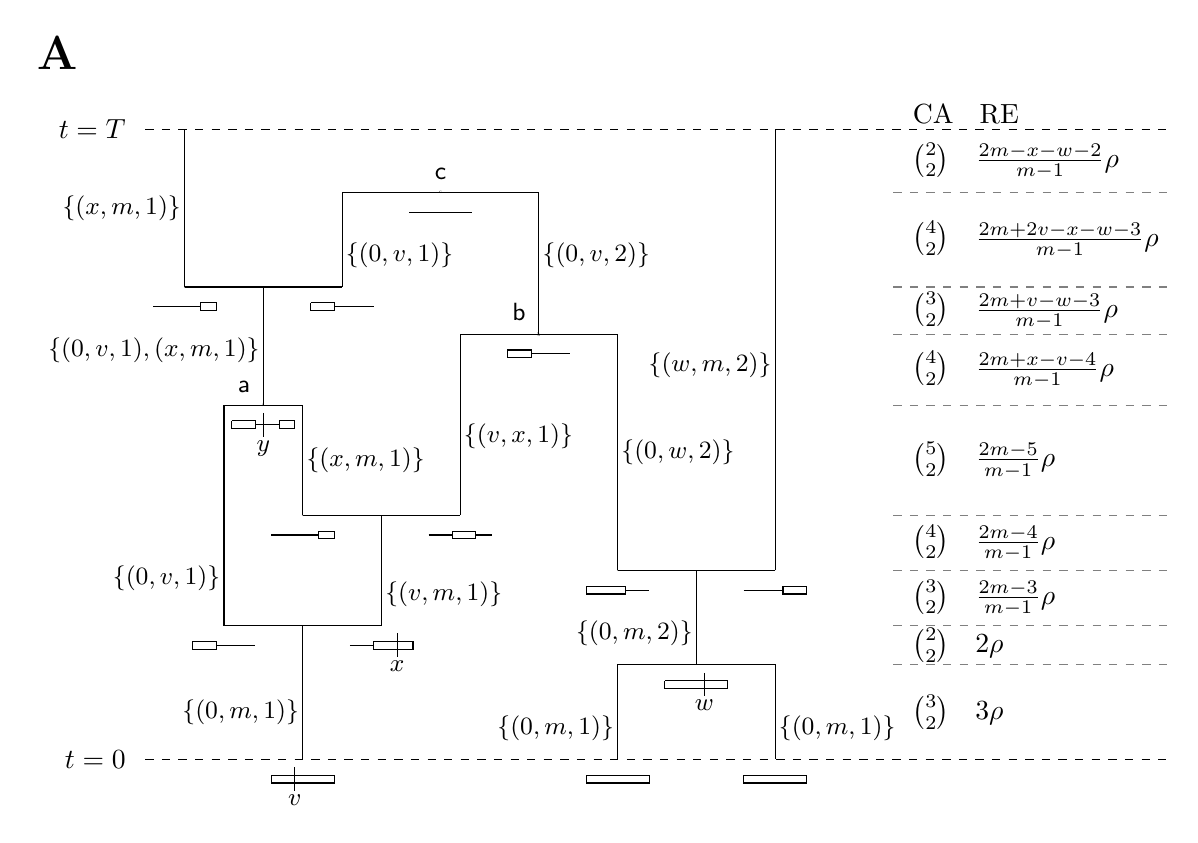
\begin{tikzpicture}
	\node [anchor=north west] at (-3.5,9.3) {\LARGE \textbf{A}};
	\draw (-0.4, -0.2) -- (0.4, -0.2) -- (0.4, -0.3) -- (-0.4, -0.3) -- (-0.4, -0.2);
	\draw (-0.1, -0.1) -- (-0.1, -0.4);
	\node [label=below:{\small $v$}] at (-0.1, -0.2) {};
	\draw (3.6, -0.2) -- (4.4, -0.2) -- (4.4, -0.3) -- (3.6, -0.3) -- (3.6, -0.2);
	\draw (5.6, -0.2) -- (6.4, -0.2) -- (6.4, -0.3) -- (5.6, -0.3) -- (5.6, -0.2);

	\draw (4,0) -- (4, 1.2) -- (6, 1.2) -- (6,0);
	\draw (4.6, 1) -- (5.4, 1) -- (5.4, 0.9) -- (4.6, 0.9) -- (4.6, 1);
	\draw (5.1, 1.1) -- (5.1, 0.8);
	\node [label=below:{\small $w$}] at (5.1, 1) {};

	\draw (0, 0) -- (0, 1.7) -- (-1,1.7) -- (1,1.7);
	\draw (-1.4, 1.5) -- (-1.1, 1.5) -- (-1.1, 1.4) -- (-1.4, 1.4) -- (-1.4, 1.5);
	\draw (-1.1, 1.45) -- (-0.6, 1.45);
	\draw (0.6, 1.45) -- (0.9, 1.45);
	\draw (0.9, 1.5) -- (1.4, 1.5) -- (1.4, 1.4) -- (0.9, 1.4) -- (0.9, 1.5);
	\draw (1.2, 1.6) -- (1.2, 1.3);
	\node [label=below:{\small $x$}] at (1.2, 1.5) {};

	\draw (5, 1.2) -- (5, 2.4) -- (4,2.4) -- (6,2.4);
	\draw (3.6, 2.2) -- (4.1, 2.2) -- (4.1, 2.1) -- (3.6, 2.1) -- (3.6, 2.2);
	\draw (4.1, 2.15) -- (4.4, 2.15);
	\draw (5.6, 2.15) -- (6.1, 2.15);
	\draw (6.1, 2.2) -- (6.4, 2.2) -- (6.4, 2.1) -- (6.1, 2.1) -- (6.1, 2.2);

	\draw (1, 1.7) -- (1, 3.1) -- (0,3.1) -- (2,3.1);
	\draw (-0.4, 2.85) -- (0.2, 2.85);
	\draw (0.2, 2.9) -- (0.4, 2.9) -- (0.4, 2.8) -- (0.2, 2.8) -- (0.2, 2.9);
	\draw (1.6, 2.85) -- (1.9, 2.85);
	\draw (1.9, 2.9) -- (2.2, 2.9) -- (2.2, 2.8) -- (1.9, 2.8) -- (1.9, 2.9);
	\draw (2.2, 2.85) -- (2.4, 2.85);

	\draw (-1, 1.7) -- (-1, 4.5) -- (0,4.5) -- (0,3.1);
	\node [scale=0.2,label=above left:{\small \textsf{a}}] at (-0.5,4.5) {a};
	\draw (-0.9, 4.3) -- (-0.6, 4.3) -- (-0.6, 4.2) -- (-0.9, 4.2) -- (-0.9, 4.3);
	\draw (-0.6, 4.25) -- (-0.3, 4.25);
	\draw (-0.3, 4.3) -- (-0.1, 4.3) -- (-0.1, 4.2) -- (-0.3, 4.2) -- (-0.3, 4.3);
	\draw (-0.5, 4.4) -- (-0.5, 4.1);
	\node [label=below:{\small $y$}] at (-0.5, 4.3) {};

	\draw (4,2.4) -- (4,5.4) -- (2,5.4) -- (2,3.1);
	\node [scale=0.2,label=above left:{\small \textsf{b}}] at (3,5.4) {b};
	\draw (2.6, 5.2) -- (2.9, 5.2) -- (2.9, 5.1) -- (2.6, 5.1) -- (2.6, 5.2);
	\draw (2.9, 5.15) -- (3.4, 5.15);

	\draw (-0.5, 4.5) -- (-0.5, 6) -- (-1.5,6) -- (0.5,6);
	\draw (-1.9, 5.75) -- (-1.3, 5.75);
	\draw (-1.3, 5.8) -- (-1.1, 5.8) -- (-1.1, 5.7) -- (-1.3, 5.7) -- (-1.3, 5.8);
	\draw (0.1, 5.8) -- (0.4, 5.8) -- (0.4, 5.7) -- (0.1, 5.7) -- (0.1, 5.8);
	\draw (0.4, 5.75) -- (0.9, 5.75);

	\draw (0.5, 6) -- (0.5, 7.2) -- (3,7.2) -- (3,5.4);
	\node [scale=0.2,label=above:{\small \textsf{c}}] at (1.75,7.2) {c};
	\draw (1.35, 6.95) -- (2.15, 6.95);

	\draw (-1.5, 6) -- (-1.5, 8);
	\draw (6, 2.4) -- (6, 8);

	% Edge annotations above each event
	\node [label=left:{\small$\{(0,m,1)\}$}] at (0.2,0.6) {};
	\node [label=left:{\small$\{(0,m,1)\}$}] at (4.2,0.4) {};
	\node [label=right:{\small$\{(0,m,1)\}$}] at (5.8,0.4) {};
	\node [label=left:{\small$\{(0,m,2)\}$}] at (5.2,1.6) {};
	\node [label=left:{\small$\{(0,v,1)\}$}] at (-0.8,2.3) {};
	\node [label=right:{\small$\{(v,m,1)\}$}] at (0.8,2.1) {};
	\node [label=right:{\small$\{(0,w,2)\}$}] at (3.8,3.9) {};
	\node [label=left:{\small$\{(w,m,2)\}$}] at (6.2,5) {};
	\node [label=right:{\small$\{(x,m,1)\}$}] at (-0.2,3.8) {};
	\node [label=right:{\small$\{(v,x,1)\}$}] at (1.8,4.1) {};
	\node [label=left:{\small$\{(0,v,1), (x,m,1)\}$}] at (-0.3,5.2) {};
	\node [label=right:{\small$\{(0,v,2)\}$}] at (2.8,6.4) {};
	\node [label=left:{\small$\{(x,m,1)\}$}] at (-1.3,7) {};
	\node [label=right:{\small$\{(0,v,1)\}$}] at (0.3,6.4) {};

	% Dashed lines for start and end times
	\draw[dashed] (-2, 0) -- (11, 0);
	\node [label=left:{$t = 0$}] at (-2,0) {};
	\draw[dashed] (-2, 8) -- (11, 8);
	\node [label=left:{$t = T$}] at (-2,8) {};

	% Numbers of extant ancestors and links, from top to bottom
	\node[label=right:{CA \; RE}] at (7.5, 8.2) {};
	\node[label=right:{$\binom{2}{2}$ \; $\frac{2 m - x - w - 2}{m - 1} \rho$}] at (7.5, 7.6) {};
	\node[label=right:{$\binom{4}{2}$ \; $\frac{2 m + 2 v - x - w - 3}{m - 1} \rho$}] at (7.5, 6.6) {};
	\node[label=right:{$\binom{3}{2}$ \; $\frac{2 m + v - w - 3}{m - 1} \rho$}] at (7.5, 5.7) {};
	\node[label=right:{$\binom{4}{2}$ \; $\frac{2 m + x - v - 4}{m - 1} \rho$}] at (7.5, 4.95) {};
	\node[label=right:{$\binom{5}{2}$ \; $\frac{2 m - 5}{m - 1} \rho$}] at (7.5, 3.8) {};
	\node[label=right:{$\binom{4}{2}$ \; $\frac{2 m - 4}{m -1} \rho$}] at (7.5, 2.75) {};
	\node[label=right:{$\binom{3}{2}$ \; $\frac{2 m - 3}{m - 1} \rho$}] at (7.5, 2.05) {};
	\node[label=right:{$\binom{2}{2}$ \; $2 \rho$}] at (7.5, 1.45) {};
	\node[label=right:{$\binom{3}{2}$ \; $3 \rho$}] at (7.5, 0.6) {};

	% Gray dashed lines to visually separate holding times
	\draw[color=gray, dashed] (7.5, 1.2) -- (11, 1.2);
	\draw[color=gray, dashed] (7.5, 1.7) -- (11, 1.7);
	\draw[color=gray, dashed] (7.5, 2.4) -- (11, 2.4);
	\draw[color=gray, dashed] (7.5, 3.1) -- (11, 3.1);
	\draw[color=gray, dashed] (7.5, 4.5) -- (11, 4.5);
	\draw[color=gray, dashed] (7.5, 5.4) -- (11, 5.4);
	\draw[color=gray, dashed] (7.5, 6) -- (11, 6);
	\draw[color=gray, dashed] (7.5, 7.2) -- (11, 7.2);
\end{tikzpicture}
&
\begin{tikzpicture}
	\node [anchor=north west] at (-3.5,9.3) {\LARGE \textbf{B}};
	\draw (-0.4, -0.2) -- (0.4, -0.2) -- (0.4, -0.3) -- (-0.4, -0.3) -- (-0.4, -0.2);
	\draw (-0.1, -0.1) -- (-0.1, -0.4);
	\node [label=below:{\small $v$}] at (-0.1, -0.2) {};
	\draw (3.6, -0.2) -- (4.4, -0.2) -- (4.4, -0.3) -- (3.6, -0.3) -- (3.6, -0.2);
	\draw (5.6, -0.2) -- (6.4, -0.2) -- (6.4, -0.3) -- (5.6, -0.3) -- (5.6, -0.2);

	\draw (4,0) -- (4, 1.2) -- (6, 1.2) -- (6,0);
	\draw (4.6, 1) -- (5.4, 1) -- (5.4, 0.9) -- (4.6, 0.9) -- (4.6, 1);
	\draw (5.1, 1.1) -- (5.1, 0.8);
	\node [label=below:{\small $w$}] at (5.1, 1) {};

	\draw (0, 0) -- (0, 1.7) -- (-1,1.7) -- (1,1.7);
	\draw (-1.4, 1.5) -- (-1.1, 1.5) -- (-1.1, 1.4) -- (-1.4, 1.4) -- (-1.4, 1.5);
	\draw (-1.1, 1.45) -- (-0.6, 1.45);
	\draw (0.6, 1.45) -- (0.9, 1.45);
	\draw (0.9, 1.5) -- (1.4, 1.5) -- (1.4, 1.4) -- (0.9, 1.4) -- (0.9, 1.5);
	\draw (1.2, 1.6) -- (1.2, 1.3);
	\node [label=below:{\small $x$}] at (1.2, 1.5) {};

	\draw (5, 1.2) -- (5, 2.4) -- (4,2.4) -- (6,2.4);
	\draw (3.6, 2.2) -- (4.1, 2.2) -- (4.1, 2.1) -- (3.6, 2.1) -- (3.6, 2.2);
	\draw (4.1, 2.15) -- (4.4, 2.15);
	\draw (5.6, 2.15) -- (6.1, 2.15);
	\draw (6.1, 2.2) -- (6.4, 2.2) -- (6.4, 2.1) -- (6.1, 2.1) -- (6.1, 2.2);
	\draw [color=red](5.8, 2.3) -- (5.8, 2.0);
	\node [label={[red]below:{\small $z$}}] at (5.8, 2.1) {};

	\draw (1, 1.7) -- (1, 3.1) -- (0,3.1) -- (2,3.1);
	\draw (-0.4, 2.85) -- (0.2, 2.85);
	\draw (0.2, 2.9) -- (0.4, 2.9) -- (0.4, 2.8) -- (0.2, 2.8) -- (0.2, 2.9);
	\draw (1.6, 2.85) -- (1.9, 2.85);
	\draw (1.9, 2.9) -- (2.2, 2.9) -- (2.2, 2.8) -- (1.9, 2.8) -- (1.9, 2.9);
	\draw (2.2, 2.85) -- (2.4, 2.85);

	\draw (-1, 1.7) -- (-1, 4.5) -- (0,4.5) -- (0,3.1);
	\draw (-0.9, 4.3) -- (-0.6, 4.3) -- (-0.6, 4.2) -- (-0.9, 4.2) -- (-0.9, 4.3);
	\draw (-0.6, 4.25) -- (-0.3, 4.25);
	\draw (-0.3, 4.3) -- (-0.1, 4.3) -- (-0.1, 4.2) -- (-0.3, 4.2) -- (-0.3, 4.3);
	\draw (-0.5, 4.4) -- (-0.5, 4.1);
	\node [label=below:{\small $y$}] at (-0.5, 4.3) {};

	\draw (6, 2.4) -- (6, 3.8) -- (7, 3.8);
	\draw [color=red](6, 3.8) -- (5, 3.8);
	\draw (4.6, 3.55) -- (5.4, 3.55);
	\draw (6.6, 3.55) -- (7.1, 3.55);
	\draw (7.1, 3.6) -- (7.4, 3.6) -- (7.4, 3.5) -- (7.1, 3.5) -- (7.1, 3.6);

	\draw (4,2.4) -- (4,5.4) -- (2,5.4) -- (2,3.1);
	\draw (2.6, 5.2) -- (2.9, 5.2) -- (2.9, 5.1) -- (2.6, 5.1) -- (2.6, 5.2);
	\draw (2.9, 5.15) -- (3.4, 5.15);

	\draw (-0.5, 4.5) -- (-0.5, 6) -- (-1.5,6) -- (0.5,6);
	\draw (-1.9, 5.75) -- (-1.3, 5.75);
	\draw (-1.3, 5.8) -- (-1.1, 5.8) -- (-1.1, 5.7) -- (-1.3, 5.7) -- (-1.3, 5.8);
	\draw (0.1, 5.8) -- (0.4, 5.8) -- (0.4, 5.7) -- (0.1, 5.7) -- (0.1, 5.8);
	\draw (0.4, 5.75) -- (0.9, 5.75);

	\draw [color=red](5, 3.8) -- (5, 6.6) -- (4, 6.6);
	\draw (4,6.6) -- (3,6.6) -- (3, 5.4);
	\draw (3.6, 6.4) -- (3.9, 6.4) -- (3.9, 6.3) -- (3.6, 6.3) -- (3.6, 6.4);
	\draw (3.9, 6.35) -- (4.4, 6.35);

	\draw (0.5, 6) -- (0.5, 7.2) -- (4,7.2) -- (4,6.6);
	\draw (1.85, 6.95) -- (2.65, 6.95);

	\draw (-1.5, 6) -- (-1.5, 8);
	\draw [color=red](2.25, 7.2) -- (2.25, 8);
	\draw (7, 3.8) -- (7, 8);

	% Dashed lines for start and end times
	\draw[dashed] (-2, 0) -- (9.1, 0);
	\node [label=left:{$t = 0$}] at (-2,0) {};
	\draw[dashed] (-2, 8) -- (9.1, 8);
	\node [label=left:{$t = T$}] at (-2,8) {};

	% Numbers of extant ancestors and links, from top to bottom
	\node[label=right:{CA \; RE}] at (7.5, 8.2) {};
	\node[label=right:{$\binom{3}{2}$ \; $3 \rho$}] at (7.5, 7.6) {};
	\node[label=right:{$\binom{4}{2}$ \; $4 \rho$}] at (7.5, 6.9) {};
	\node[label=right:{$\binom{5}{2}$ \; $5 \rho$}] at (7.5, 6.3) {};
	\node[label=right:{$\binom{4}{2}$ \; $4 \rho$}] at (7.5, 5.7) {};
	\node[label=right:{$\binom{5}{2}$ \; $5 \rho$}] at (7.5, 4.95) {};
	\node[label=right:{$\binom{6}{2}$ \; $6 \rho$}] at (7.5, 4.15) {};
	\node[label=right:{$\binom{5}{2}$ \; $5 \rho$}] at (7.5, 3.45) {};
	\node[label=right:{$\binom{4}{2}$ \; $4 \rho$}] at (7.5, 2.75) {};
	\node[label=right:{$\binom{3}{2}$ \; $3 \rho$}] at (7.5, 2.05) {};
	\node[label=right:{$\binom{2}{2}$ \; $2 \rho$}] at (7.5, 1.45) {};
	\node[label=right:{$\binom{3}{2}$ \; $3 \rho$}] at (7.5, 0.6) {};

	% Gray dashed lines to visually separate holding times
	\draw[color=gray, dashed] (7.5, 1.2) -- (9.1, 1.2);
	\draw[color=gray, dashed] (7.5, 1.7) -- (9.1, 1.7);
	\draw[color=gray, dashed] (7.5, 2.4) -- (9.1, 2.4);
	\draw[color=gray, dashed] (7.5, 3.1) -- (9.1, 3.1);
	\draw[color=gray, dashed] (7.5, 3.8) -- (9.1, 3.8);
	\draw[color=gray, dashed] (7.5, 4.5) -- (9.1, 4.5);
	\draw[color=gray, dashed] (7.5, 5.4) -- (9.1, 5.4);
	\draw[color=gray, dashed] (7.5, 6) -- (9.1, 6);
	\draw[color=gray, dashed] (7.5, 6.6) -- (9.1, 6.6);
	\draw[color=gray, dashed] (7.5, 7.2) -- (9.1, 7.2);
\end{tikzpicture}
\end{tabular}
}
\caption{(A)
A realisation of the graph traversed by Hudson's algorithm started from a
sample of three chromosomes of length $m$ at time $t = 0$, and
propagated until time $T$. The MRCA on the genetic interval $[v, w)$ is reached
at event \textsf{b}, while that on $[0, v)$ is reached at event \textsf{c}.
The non-ancestral segment $[v, w)$ above
A contributes to the rate of effective recombinations because it
is trapped between ancestral segments. The two columns titled CA and RE
are the respective rates of mergers and recombinations when
the recombination rate is $\rho$.
(B) A corresponding realisation of a big ARG, which augments Hudson's algorithm
by tracking nonancestral lineages. The result is a simpler state space and
dynamics, at the cost of extra nodes and edges, highlighted in red, which do
not affect the local tree at any site.}
\label{hudson_vs_bigARG}
\end{figure}

% Full quote:
% This process simplifies mathematics on the account that the notion of an
% ancestor will have a less restrictive meaning than usual:
% An ``ancestral'' sequence in the birth and death process
% need not have any genetic material in common with a
% sequence descended from it.

\section{Survey of ARG inference methods}

The problem of reconstructing ARGs for samples of recombining sequences has
been of interest since the ARG was first defined. Early methods focused on
finding \emph{parsimonious} ARGs, i.e.\ those with a minimal number of
recombination events \citep{hein1990reconstructing}. Two main approaches
emerged: \emph{backwards-in-time} \citep{lyngso2005minimum} and
\emph{along-the-genome} \citep{song2003parsimonious, song2005constructing}. The
former starts with a data matrix and reduces it to an empty matrix through row
and column operations corresponding to coalescence, mutation, and recombination
events, which construct an ARG from the bottom up. The latter begins from an
initial local tree at a single focal site. Moving the focal site along the
genome changes the local tree via a \emph{subtree prune and regraft} (SPR)
operation whenever a recombination is encountered. Methods based the
backwards-in-time approach are described by \citet{song2005efficient,
wu2008association, thao2019hybrid, ignatieva2021kwarg}, while
\citet{hein1993heuristic, wu2011new, mirzaei2017rent} describe along-the-genome
methods. \citet{rasmussen2022espalier} focuses on parsimonious fusion of local
trees into an ARG, while \citet{camara2016inference} is based on topological
data analysis.

Reconstructing a most parsimonious ARG for a given data set is NP-hard
\citep{wang2001perfect}, so parsimony-based methods resort to heuristics and
are limited to analysing at most hundreds of sequences. Hence, a number of
methods aim to balance computational efficiency with reconstruction of
``reasonable", rather than parsimonious ARGs \citep{minichiello2006mapping,
parida2008estimating, kelleher2019inferring,  speidel2019method,
zhang2023biobank}. The latter three methods, as well as the parsimony-based
method of \citet{rasmussen2022espalier}, can be used on megabase scale data and
hundreds of thousands of samples under human-like parameters.

TODO mention \citep{schaefer2021ancestral} somewhere.
Also \citep{kuhner2017consensus}.

% AI: just to note, these papers do not all agree in their definition of an
% ARG. I guess this is one of the points of the present paper, but should we
% mention this fact? Should we also mention that most of these infer just the
% topology, but some also the times?

An alternative approach is to treat the ARG as a latent parameter to be
averaged out by Monte Carlo methods, based either on importance sampling
\citep{griffiths1996ancestral, fearnhead2001estimating, jenkins2011inference}
or MCMC \citep{kuhner2000maximum, nielsen2000estimation, wang2008bayesian,
fallon2013acg, mahmoudi2022bayesian}. These methods operate on representations
of the ``little ARG'', and are extremely computationally expensive, being
applicable to at most hundreds of samples consisting of tens or hundreds of
kilobases with human-like parameters. State-of-the-art methods rely on cheaper,
approximate models \citep{didelot2010inference, heine2018bridging,
hubisz2020mapping,hubisz2020inference, medina2020speeding}. The most scalable
method, \texttt{ARGWeaver} \citep{rasmussen2014genome}, can be applied to
dozens of mammal-like genomes \citep{hubisz2020inference}. A central quantity
in all of these sampling methods is the conditional sampling probability $p(G |
D) \propto p(D | G) p(G)$ of an ARG $G$ given an observed realization of
genetic diversity $D$ at its sampled leaves, where $p(D | G)$ is the likelihood
of the data $D$ given $G$, and $p(G)$ is a Bayesian prior distribution or a
frequentist regularizer for the ARG $G$.

The likelihood $p(D | G)$ is effectively always the distribution of a Poisson
process on the ancestral material along the edges of $G$ \citep[Eq.\
(2)]{mahmoudi2022bayesian}. Hence it is typically straightforward to evaluate
in principle, but choosing the right data structure can still have a dramatic
effect on the efficiency of evaluation \citep{mahmoudi2022bayesian}. Especially
in the Bayesian case, $p(G)$ is typically specified as the sampling
distribution of a stochastic process, such as the coalescent with
recombination. Two contemporary examples are \cite{mahmoudi2022bayesian,
guo2022recombination}. Evaluating the distribution of the coalescent with
recombination (or related models) requires knowledge of the number of extant
lineages and number of links available for recombination (i.e.\ ones at which a
recombination would split ancestral material) at each time \citep[Eq.\
(3)]{mahmoudi2022bayesian}. These require a data structure from which shared
edges on different trees are easy to identify, and which encodes recombination
events and times explicitly, e.g.\ using nodes.
We will provide a more detailed discussion on sampling probability evaluation in the appendix.
\end{document}
